\chapter{Deep Learning in Structured Domains} \label{ch:deep-learning-structures}
A \keyword{structured domain} is a data domain whose elements are formed by a set of atomic \emph{entities}, and the \emph{relations} between them. Structured data is common in several fields, such as biology, chemistry, finance, social networks, and many more. Typical examples are sequences such as time-series data, or graphs representing molecular structures. One distinctive characteristic of structured data is that it has \keyword{variable size}, meaning that the number of entities composing the datum is not fixed in general. This constitutes a serious limitation for traditional \gls{ml} models, which are designed to work with \quotes{flat} data, \ie collections of fixed-size vectors. In principle, they can be adapted to work with variable-sized data by incorporating the structure of the data to the input vectors as additional features. While useful to some extent, this approach requires to decide \apriori which features are needed to solve a task. This, in turn, requires a level of domain expertise that is not always available for many interesting problems. In contrast, \glspl{nn} (and Deep Learning models more so) are able to learn which features are useful to solve a task adaptively from data, without the need of feature engineering. Thus, the general idea is to provide the structured data directly as an input to the network, which automatically learns the needed features and the task, guided by the learning process. In this chapter, we present a class of \glspl{nn} that are able to handle variable-sized inputs for learning in structured domains.

\section{Graphs}\label{sec:graphs}
The elements of structured domains can be described in a compact and convenient notation using the general formalism of \keyword{graphs}. Informally, a graph is a collection of \emph{vertices} (the entities) connected through a collection of \emph{edges} (the relations). In literature, vertices are sometimes called \emph{nodes}, while edges are also referred to as \emph{arcs} or \emph{links}. Formally, a graph with $n$ vertices a pair
$$G =\langle \Cal{V}_G, \Cal{E}_G \rangle,$$
where $\Cal{V}_G = \Set{v_1, v_2, \ldots, v_n}$ is its set of vertices, and $\Cal{E}_G = \{\{u, v\} \mid u, v \in \Cal{V}_G\}$ is its set of edges. In a graph, $\Cal{E}_G$  specifies the graph \emph{structure}, that is, the way vertices and edges are interconnected. Notice that the pair $\Set{u,v}$ is unordered: in this case, the graph is called \keyword{undirected}. Figure \ref{fig:undirected-graph} shows a visual representation of an undirected graph.
Given an edge $\Set{u, v} \in \Cal{E}_G$, $u$ and $v$ are called its \emph{endpoints}, and are said to be \emph{adjacent}. Alternatively, we say that $\Set{u, v}$ is \emph{incident} to $u$ and $v$. Edges of the form $\Set{v,v}$ that connect a vertex to itself are called \emph{self-loops}.
\begin{figure*}
    \begin{subfigure}[b]{0.38\linewidth}
        \centering
        \resizebox{.8\textwidth}{!}{

\tikzset{every picture/.style={line width=0.75pt}} %set default line width to 0.75pt        

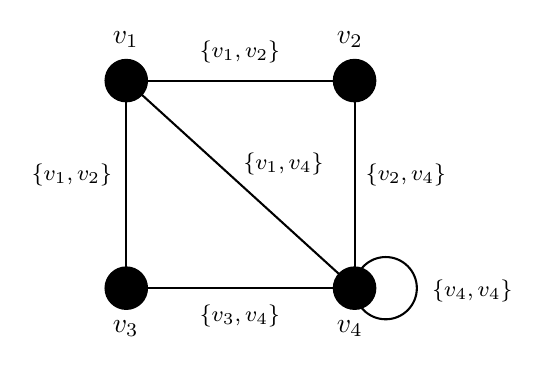
\begin{tikzpicture}[x=0.75pt,y=0.75pt,yscale=-1,xscale=1]
%uncomment if require: \path (0,178); %set diagram left start at 0, and has height of 178

%Shape: Circle [id:dp07024740871786728] 
\draw  [color={rgb, 255:red, 0; green, 0; blue, 0 }  ,draw opacity=1 ][fill={rgb, 255:red, 0; green, 0; blue, 0 }  ,fill opacity=1 ] (70,40) .. controls (70,34.48) and (74.48,30) .. (80,30) .. controls (85.52,30) and (90,34.48) .. (90,40) .. controls (90,45.52) and (85.52,50) .. (80,50) .. controls (74.48,50) and (70,45.52) .. (70,40) -- cycle ;
%Shape: Circle [id:dp433131734933478] 
\draw  [color={rgb, 255:red, 0; green, 0; blue, 0 }  ,draw opacity=1 ][fill={rgb, 255:red, 0; green, 0; blue, 0 }  ,fill opacity=1 ] (180,140) .. controls (180,134.48) and (184.48,130) .. (190,130) .. controls (195.52,130) and (200,134.48) .. (200,140) .. controls (200,145.52) and (195.52,150) .. (190,150) .. controls (184.48,150) and (180,145.52) .. (180,140) -- cycle ;
%Straight Lines [id:da2632273187556222] 
\draw    (80,40) -- (190,40) ;
%Straight Lines [id:da44290236983487796] 
\draw    (80,40) -- (80,140) ;
%Straight Lines [id:da1506700219779713] 
\draw    (80,40) -- (190,140) ;
%Straight Lines [id:da22133122848697484] 
\draw    (190,140) -- (190,40) ;
%Straight Lines [id:da5021664543420994] 
\draw    (80,140) -- (190,140) ;
%Shape: Circle [id:dp5653232034601401] 
\draw  [color={rgb, 255:red, 0; green, 0; blue, 0 }  ,draw opacity=1 ][fill={rgb, 255:red, 0; green, 0; blue, 0 }  ,fill opacity=1 ] (180,40) .. controls (180,34.48) and (184.48,30) .. (190,30) .. controls (195.52,30) and (200,34.48) .. (200,40) .. controls (200,45.52) and (195.52,50) .. (190,50) .. controls (184.48,50) and (180,45.52) .. (180,40) -- cycle ;
%Shape: Circle [id:dp644957096812665] 
\draw   (190,140) .. controls (190,131.72) and (196.72,125) .. (205,125) .. controls (213.28,125) and (220,131.72) .. (220,140) .. controls (220,148.28) and (213.28,155) .. (205,155) .. controls (196.72,155) and (190,148.28) .. (190,140) -- cycle ;
%Shape: Circle [id:dp5636675532432875] 
\draw  [color={rgb, 255:red, 0; green, 0; blue, 0 }  ,draw opacity=1 ][fill={rgb, 255:red, 0; green, 0; blue, 0 }  ,fill opacity=1 ] (70,140) .. controls (70,134.48) and (74.48,130) .. (80,130) .. controls (85.52,130) and (90,134.48) .. (90,140) .. controls (90,145.52) and (85.52,150) .. (80,150) .. controls (74.48,150) and (70,145.52) .. (70,140) -- cycle ;

% Text Node
\draw (72,15) node [anchor=north west][inner sep=0.75pt]    {$v_{1}$};
% Text Node
\draw (180,15) node [anchor=north west][inner sep=0.75pt]    {$v_{2}$};
% Text Node
\draw (72,154) node [anchor=north west][inner sep=0.75pt]    {$v_{3}$};
% Text Node
\draw (180,154) node [anchor=north west][inner sep=0.75pt]    {$v_{4}$};
% Text Node
\draw (114,19.4) node [anchor=north west][inner sep=0.75pt]  [font=\footnotesize]  {$\{v_{1} ,v_{2}\}$};
% Text Node
\draw (135,73.4) node [anchor=north west][inner sep=0.75pt]  [font=\footnotesize]  {$\{v_{1} ,v_{4}\}$};
% Text Node
\draw (194,78.4) node [anchor=north west][inner sep=0.75pt]  [font=\footnotesize]  {$\{v_{2} ,v_{4}\}$};
% Text Node
\draw (33,78.4) node [anchor=north west][inner sep=0.75pt]  [font=\footnotesize]  {$\{v_{1} ,v_{2}\}$};
% Text Node
\draw (114,146.4) node [anchor=north west][inner sep=0.75pt]  [font=\footnotesize]  {$\{v_{3} ,v_{4}\}$};
% Text Node
\draw (226,134.4) node [anchor=north west][inner sep=0.75pt]  [font=\footnotesize]  {$\{v_{4} ,v_{4}\}$};


\end{tikzpicture}}
        \caption{An undirected graph.}
        \label{fig:undirected-graph}
    \end{subfigure}
    \begin{subfigure}[b]{0.32\linewidth}
        \centering
        \resizebox{.8\textwidth}{!}{

\tikzset{every picture/.style={line width=0.75pt}} %set default line width to 0.75pt

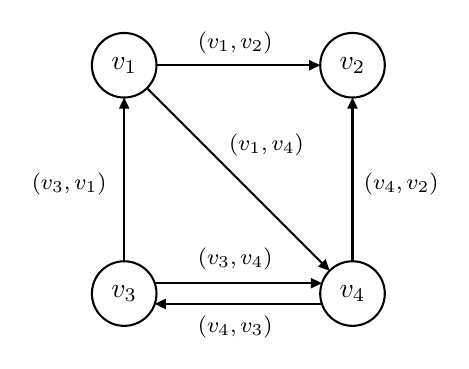
\begin{tikzpicture}[x=0.75pt,y=0.75pt,yscale=-1,xscale=1]
%uncomment if require: \path (0,186); %set diagram left start at 0, and has height of 186


% Text Node
\draw (314,12.4) node [anchor=north west][inner sep=0.75pt]  [font=\footnotesize]  {$( v_{1} ,v_{2})$};
% Text Node
\draw    (280, 30) circle [x radius= 15.56, y radius= 15.56]   ;
\draw (280,30) node   [align=left] {\begin{minipage}[lt]{13.600000000000001pt}\setlength\topsep{0pt}
\begin{center}
$\displaystyle v_{1}$
\end{center}

\end{minipage}};
% Text Node
\draw    (390, 30) circle [x radius= 15.56, y radius= 15.56]   ;
\draw (390,30) node   [align=left] {\begin{minipage}[lt]{13.600000000000001pt}\setlength\topsep{0pt}
\begin{center}
$\displaystyle v_{2}$
\end{center}

\end{minipage}};
% Text Node
\draw    (280, 140) circle [x radius= 15.56, y radius= 15.56]   ;
\draw (280,140) node   [align=left] {\begin{minipage}[lt]{13.600000000000001pt}\setlength\topsep{0pt}
\begin{center}
$\displaystyle v_{3}$
\end{center}

\end{minipage}};
% Text Node
\draw    (390, 140) circle [x radius= 15.56, y radius= 15.56]   ;
\draw (390,140) node   [align=left] {\begin{minipage}[lt]{13.600000000000001pt}\setlength\topsep{0pt}
\begin{center}
$\displaystyle v_{4}$
\end{center}

\end{minipage}};
% Text Node
\draw (314,149.4) node [anchor=north west][inner sep=0.75pt]  [font=\footnotesize]  {$( v_{4} ,v_{3})$};
% Text Node
\draw (314,116.4) node [anchor=north west][inner sep=0.75pt]  [font=\footnotesize]  {$( v_{3} ,v_{4})$};
% Text Node
\draw (329,61.4) node [anchor=north west][inner sep=0.75pt]  [font=\footnotesize]  {$( v_{1} ,v_{4})$};
% Text Node
\draw (394,80.4) node [anchor=north west][inner sep=0.75pt]  [font=\footnotesize]  {$( v_{4} ,v_{2})$};
% Text Node
\draw (234,80.4) node [anchor=north west][inner sep=0.75pt]  [font=\footnotesize]  {$( v_{3} ,v_{1})$};
% Connection
\draw    (280,124.44) -- (280,48.56) ;
\draw [shift={(280,45.56)}, rotate = 450] [fill={rgb, 255:red, 0; green, 0; blue, 0 }  ][line width=0.08]  [draw opacity=0] (5.36,-2.57) -- (0,0) -- (5.36,2.57) -- cycle    ;
% Connection
\draw    (295.56,30) -- (371.44,30) ;
\draw [shift={(374.44,30)}, rotate = 180] [fill={rgb, 255:red, 0; green, 0; blue, 0 }  ][line width=0.08]  [draw opacity=0] (5.36,-2.57) -- (0,0) -- (5.36,2.57) -- cycle    ;
% Connection
\draw    (291,41) -- (376.88,126.88) ;
\draw [shift={(379,129)}, rotate = 225] [fill={rgb, 255:red, 0; green, 0; blue, 0 }  ][line width=0.08]  [draw opacity=0] (5.36,-2.57) -- (0,0) -- (5.36,2.57) -- cycle    ;
% Connection
\draw    (390,124.44) -- (390,48.56) ;
\draw [shift={(390,45.56)}, rotate = 450] [fill={rgb, 255:red, 0; green, 0; blue, 0 }  ][line width=0.08]  [draw opacity=0] (5.36,-2.57) -- (0,0) -- (5.36,2.57) -- cycle    ;
% Connection
\draw    (375.26,145) -- (297.74,145) ;
\draw [shift={(294.74,145)}, rotate = 360] [fill={rgb, 255:red, 0; green, 0; blue, 0 }  ][line width=0.08]  [draw opacity=0] (5.36,-2.57) -- (0,0) -- (5.36,2.57) -- cycle    ;
% Connection
\draw    (294.74,135) -- (372.26,135) ;
\draw [shift={(375.26,135)}, rotate = 180] [fill={rgb, 255:red, 0; green, 0; blue, 0 }  ][line width=0.08]  [draw opacity=0] (5.36,-2.57) -- (0,0) -- (5.36,2.57) -- cycle    ;

\end{tikzpicture}}
        \caption{A directed graph.}
        \label{fig:directed-graph}
    \end{subfigure}
    \begin{subfigure}[b]{0.25\linewidth}
        \centering
        \resizebox{.9\textwidth}{!}{

\tikzset{every picture/.style={line width=0.75pt}} %set default line width to 0.75pt        

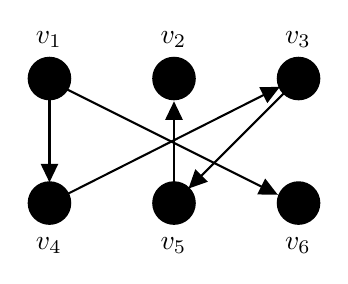
\begin{tikzpicture}[x=0.75pt,y=0.75pt,yscale=-1,xscale=1]
%uncomment if require: \path (0,144); %set diagram left start at 0, and has height of 144

%Straight Lines [id:da7193850870149698] 
\draw    (40,42) -- (40,88) ;
\draw [shift={(40,91)}, rotate = 270] [fill={rgb, 255:red, 0; green, 0; blue, 0 }  ][line width=0.08]  [draw opacity=0] (8.93,-4.29) -- (0,0) -- (8.93,4.29) -- cycle    ;
%Straight Lines [id:da1942442489782492] 
\draw    (40,42) -- (147.32,95.66) ;
\draw [shift={(150,97)}, rotate = 206.57] [fill={rgb, 255:red, 0; green, 0; blue, 0 }  ][line width=0.08]  [draw opacity=0] (8.93,-4.29) -- (0,0) -- (8.93,4.29) -- cycle    ;
%Straight Lines [id:da810447408180448] 
\draw    (100,92) -- (100,55) ;
\draw [shift={(100,52)}, rotate = 450] [fill={rgb, 255:red, 0; green, 0; blue, 0 }  ][line width=0.08]  [draw opacity=0] (8.93,-4.29) -- (0,0) -- (8.93,4.29) -- cycle    ;
%Straight Lines [id:da5553980379264378] 
\draw    (160,41) -- (109.12,91.88) ;
\draw [shift={(107,94)}, rotate = 315] [fill={rgb, 255:red, 0; green, 0; blue, 0 }  ][line width=0.08]  [draw opacity=0] (8.93,-4.29) -- (0,0) -- (8.93,4.29) -- cycle    ;
%Shape: Circle [id:dp8635781174027584] 
\draw  [color={rgb, 255:red, 0; green, 0; blue, 0 }  ,draw opacity=1 ][fill={rgb, 255:red, 0; green, 0; blue, 0 }  ,fill opacity=1 ] (30,41) .. controls (30,35.48) and (34.48,31) .. (40,31) .. controls (45.52,31) and (50,35.48) .. (50,41) .. controls (50,46.52) and (45.52,51) .. (40,51) .. controls (34.48,51) and (30,46.52) .. (30,41) -- cycle ;
%Shape: Circle [id:dp5046309407375] 
\draw  [color={rgb, 255:red, 0; green, 0; blue, 0 }  ,draw opacity=1 ][fill={rgb, 255:red, 0; green, 0; blue, 0 }  ,fill opacity=1 ] (90,41) .. controls (90,35.48) and (94.48,31) .. (100,31) .. controls (105.52,31) and (110,35.48) .. (110,41) .. controls (110,46.52) and (105.52,51) .. (100,51) .. controls (94.48,51) and (90,46.52) .. (90,41) -- cycle ;
%Shape: Circle [id:dp9523637573320518] 
\draw  [color={rgb, 255:red, 0; green, 0; blue, 0 }  ,draw opacity=1 ][fill={rgb, 255:red, 0; green, 0; blue, 0 }  ,fill opacity=1 ] (150,41) .. controls (150,35.48) and (154.48,31) .. (160,31) .. controls (165.52,31) and (170,35.48) .. (170,41) .. controls (170,46.52) and (165.52,51) .. (160,51) .. controls (154.48,51) and (150,46.52) .. (150,41) -- cycle ;
%Shape: Circle [id:dp46076804005955263] 
\draw  [color={rgb, 255:red, 0; green, 0; blue, 0 }  ,draw opacity=1 ][fill={rgb, 255:red, 0; green, 0; blue, 0 }  ,fill opacity=1 ] (30,101) .. controls (30,95.48) and (34.48,91) .. (40,91) .. controls (45.52,91) and (50,95.48) .. (50,101) .. controls (50,106.52) and (45.52,111) .. (40,111) .. controls (34.48,111) and (30,106.52) .. (30,101) -- cycle ;
%Shape: Circle [id:dp780817892587097] 
\draw  [color={rgb, 255:red, 0; green, 0; blue, 0 }  ,draw opacity=1 ][fill={rgb, 255:red, 0; green, 0; blue, 0 }  ,fill opacity=1 ] (90,101) .. controls (90,95.48) and (94.48,91) .. (100,91) .. controls (105.52,91) and (110,95.48) .. (110,101) .. controls (110,106.52) and (105.52,111) .. (100,111) .. controls (94.48,111) and (90,106.52) .. (90,101) -- cycle ;
%Shape: Circle [id:dp33231757908254456] 
\draw  [color={rgb, 255:red, 0; green, 0; blue, 0 }  ,draw opacity=1 ][fill={rgb, 255:red, 0; green, 0; blue, 0 }  ,fill opacity=1 ] (150,101) .. controls (150,95.48) and (154.48,91) .. (160,91) .. controls (165.52,91) and (170,95.48) .. (170,101) .. controls (170,106.52) and (165.52,111) .. (160,111) .. controls (154.48,111) and (150,106.52) .. (150,101) -- cycle ;
%Straight Lines [id:da4251496567702082] 
\draw    (40,101) -- (148.32,46.35) ;
\draw [shift={(151,45)}, rotate = 513.23] [fill={rgb, 255:red, 0; green, 0; blue, 0 }  ][line width=0.08]  [draw opacity=0] (8.93,-4.29) -- (0,0) -- (8.93,4.29) -- cycle    ;

% Text Node
\draw (32,17) node [anchor=north west][inner sep=0.75pt]    {$v_{1}$};
% Text Node
\draw (92,17) node [anchor=north west][inner sep=0.75pt]    {$v_{2}$};
% Text Node
\draw (152,17) node [anchor=north west][inner sep=0.75pt]    {$v_{3}$};
% Text Node
\draw (32,116) node [anchor=north west][inner sep=0.75pt]    {$v_{4}$};
% Text Node
\draw (92,116) node [anchor=north west][inner sep=0.75pt]    {$v_{5}$};
% Text Node
\draw (152,116) node [anchor=north west][inner sep=0.75pt]    {$v_{6}$};


\end{tikzpicture}}
        \caption{A bipartite graph.}
        \label{fig:bipartite-graph}
    \end{subfigure}
    \caption{Three examples of graphs.}
\end{figure*}
Graphs where it is possible to have more than one edge between a pair of vertices are called \emph{multigraphs}. In this work, we restrict ourselves to the case where there is at most one possible edge between two vertices.

\paragraph{Directed Graphs}
A \keyword{directed graph} is one where he edges are ordered pairs of vertices, or equivalently one where $\Cal{E}_G \subseteq \Cal{V}_G \times \Cal{V}_G$. A directed edge is written as $(u, v)$, meaning that it goes from vertex $u$ to vertex $v$. An example of directed graph is shown in Figure \ref{fig:directed-graph}. Given a directed graph $G$ and one of its vertices $v$, the set of all vertices from which an edge reaches $v$ is called \emph{predecessors} set, and is defined as $\Cal{P}(v) = \{u \in \Cal{V} \mid (u,v) \in \Cal{E}\}$. The cardinality of the predecessors set is called the \emph{in-degree} of the vertex, and we indicate it as $\Fun{degree}_{in}(v)$. Analogously, the set of all vertices reached by an edge from $v$ is called the \emph{successors} set, and is defined as $\Cal{s}(v) = \{u \in \Cal{V}_G \mid (v,u) \in \Cal{E}_G\}$. Its cardinality is called the \emph{out-degree} of the vertex, and indicated as $\Fun{degree}_{out}(v)$. The \emph{neighborhood} (or \emph{adjacency set}) of a vertex $v$ is the union of the predecessors and successors sets: $\Cal{N}(v) = \Cal{P}(v) \bigcup \Cal{s}(v)$. Alternatively, one can view the neighborhood as a function $\Cal{N}: \Cal{V}_G \shortrightarrow 2^{\Cal{V}_G}$ from vertices to sets of vertices. The cardinality of the neighborhood is called the \keyword{degree} of the vertex, indicated as $\Fun{degree}(v)$.  In this work, we consider all graphs directed unless otherwise specified. Undirected graphs are thus implicitly transformed into directed graphs with the same vertices, where the set of edges contains the edges $(v,u)$ and $(u,v)$ if and only if $\{u,v\}$ is an edge of the undirected graph.

\paragraph{Bipartite Graphs}
A graph $G$ is called \keyword{bipartite} if we can split $\Cal{V}_G$ in two disjoint subsets $\Cal{V}_G^{+}$ and $\Cal{V}_G^{-}$, such that $(u, v) \in \Cal{E}_G$ if and only if either $u \in \Cal{V}_G^{+}$ and $v \in \Cal{V}_G^{-}$, or $v \in \Cal{V}_G^{+}$ and $u \in \Cal{V}_G^{-}$. Figure \ref{fig:bipartite-graph} shows an example of bipartite graph, where
$\Cal{V}_G^{+} = \Set{v_1, v_2, v_3}$ and $\Cal{V}_G^{-} = \Set{v_4, v_5, v_6}$.

\paragraph{Walks, Paths, and Cycles}
Let $G$ be a graph. A \emph{walk} of length $l$ is any sequence of $l$ vertices $\Seq{v_1, v_2, \ldots, v_l}$, where each pair of consecutive vertices is adjacent, \ie $\Seq{v_i, v_{i+1}} \in \Cal{E}_G$, $\forall i= 1, \ldots, i-1$. A \emph{path} of length $l$ from vertex $u$ to vertex $v$ is a walk such that $v_1 = u$ and $v_l = v$, where each vertex appears exactly once in the sequence. If, given two vertices $u, v \in \Cal{V}_G$ such that $u \neq v$, there exists a path between them, we say they are \emph{connected}, or that $v$ is reachable from $u$. Otherwise, we say they are \emph{disconnected}, or that $v$ is unreachable from $u$. A graph is called \emph{connected} if every vertex is connected to any other vertex (ignoring the direction of the edges); otherwise it is called \emph{disconnected}. A \emph{cycle}, or \emph{loop}, of length $l$ is a walk where $v_1 = v_l$, and all the other vertices appear once in the sequence. Graphs that do not contain cycles are called \emph{acyclic}. 

\paragraph{Trees and Sequences}
A graph $T$ is called a \keyword{tree} if its set of edges defines a \emph{partial order} over the set of vertices, implying that it is also connected and acyclic. The vertices of a tree are called \emph{nodes}. Given an edge $(u, v) \in \Cal{E}_T$, we call $u$ the \emph{parent} of $v$ and $v$ the \emph{child} of $u$. The set of children of a node $v$ is indicated with the notation $\Fun{ch}(v)$. In a tree, every node has exactly one parent, with the exception of a node called \emph{root} or \emph{supersource}, which has no parent node. A tree is \emph{positional} if we can distinguish among the children of a node, \ie if there exist a consistent ordering between them. Trees have a recursive structure: every node $v \in \Cal{V}_T$ is itself the root of a tree, called \emph{sub-tree of T rooted at v}, and indicated as $S(v)$. If $S(v)$ contains only $v$, $v$ is called a \emph{leaf}. Trees encode \emph{hierarchical} relationships among nodes; an example of tree with five nodes is shown in Figure \ref{fig:tree}. 

A graph $S$ with $n$ vertices is called a \emph{sequential graph}, or \keyword{sequence} of length $n$, if its set of edges defines a \emph{total order} over the set of vertices, which allows us to represent the set of vertices in an ordered fashion as $\Cal{V}_S = (v_1, v_2, \ldots, v_n)$. In a sequence, the vertices are usually called \emph{elements}. A sequence can be viewed as a special case of tree with only one leaf. Sequences are useful to encode \emph{sequential} relationships among elements; Figure \ref{fig:sequence} shows an example of a sequence of four elements. 
\begin{figure*}
    \begin{subfigure}[b]{0.49\linewidth}
        \centering
        \resizebox{.8\textwidth}{!}{

\tikzset{every picture/.style={line width=0.75pt}} %set default line width to 0.75pt        

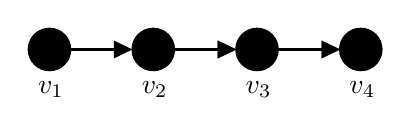
\begin{tikzpicture}[x=0.75pt,y=0.75pt,yscale=-1,xscale=1]
%uncomment if require: \path (0,54); %set diagram left start at 0, and has height of 54

%Shape: Circle [id:dp5966637236046903] 
\draw  [fill={rgb, 255:red, 0; green, 0; blue, 0 }  ,fill opacity=1 ] (10,20) .. controls (10,14.48) and (14.48,10) .. (20,10) .. controls (25.52,10) and (30,14.48) .. (30,20) .. controls (30,25.52) and (25.52,30) .. (20,30) .. controls (14.48,30) and (10,25.52) .. (10,20) -- cycle ;
%Straight Lines [id:da052084780507878126] 
\draw    (20,20) -- (57,20) ;
\draw [shift={(60,20)}, rotate = 180] [fill={rgb, 255:red, 0; green, 0; blue, 0 }  ][line width=0.08]  [draw opacity=0] (8.93,-4.29) -- (0,0) -- (8.93,4.29) -- cycle    ;
%Shape: Circle [id:dp5200693045335503] 
\draw  [fill={rgb, 255:red, 0; green, 0; blue, 0 }  ,fill opacity=1 ] (60,20) .. controls (60,14.48) and (64.48,10) .. (70,10) .. controls (75.52,10) and (80,14.48) .. (80,20) .. controls (80,25.52) and (75.52,30) .. (70,30) .. controls (64.48,30) and (60,25.52) .. (60,20) -- cycle ;
%Straight Lines [id:da33269281061881717] 
\draw    (70,20) -- (107,20) ;
\draw [shift={(110,20)}, rotate = 180] [fill={rgb, 255:red, 0; green, 0; blue, 0 }  ][line width=0.08]  [draw opacity=0] (8.93,-4.29) -- (0,0) -- (8.93,4.29) -- cycle    ;
%Straight Lines [id:da9716435563701427] 
\draw    (70,20) -- (107,20) ;
\draw [shift={(110,20)}, rotate = 180] [fill={rgb, 255:red, 0; green, 0; blue, 0 }  ][line width=0.08]  [draw opacity=0] (8.93,-4.29) -- (0,0) -- (8.93,4.29) -- cycle    ;
%Shape: Circle [id:dp3815536377212252] 
\draw  [fill={rgb, 255:red, 0; green, 0; blue, 0 }  ,fill opacity=1 ] (110,20) .. controls (110,14.48) and (114.48,10) .. (120,10) .. controls (125.52,10) and (130,14.48) .. (130,20) .. controls (130,25.52) and (125.52,30) .. (120,30) .. controls (114.48,30) and (110,25.52) .. (110,20) -- cycle ;
%Straight Lines [id:da660694621597677] 
\draw    (120,20) -- (157,20) ;
\draw [shift={(160,20)}, rotate = 180] [fill={rgb, 255:red, 0; green, 0; blue, 0 }  ][line width=0.08]  [draw opacity=0] (8.93,-4.29) -- (0,0) -- (8.93,4.29) -- cycle    ;
%Straight Lines [id:da23904459539502287] 
\draw    (120,20) -- (157,20) ;
\draw [shift={(160,20)}, rotate = 180] [fill={rgb, 255:red, 0; green, 0; blue, 0 }  ][line width=0.08]  [draw opacity=0] (8.93,-4.29) -- (0,0) -- (8.93,4.29) -- cycle    ;
%Shape: Circle [id:dp3652036582720466] 
\draw  [fill={rgb, 255:red, 0; green, 0; blue, 0 }  ,fill opacity=1 ] (160,20) .. controls (160,14.48) and (164.48,10) .. (170,10) .. controls (175.52,10) and (180,14.48) .. (180,20) .. controls (180,25.52) and (175.52,30) .. (170,30) .. controls (164.48,30) and (160,25.52) .. (160,20) -- cycle ;

% Text Node
\draw (13,34) node [anchor=north west][inner sep=0.75pt]    {$v_1$};
% Text Node
\draw (63,34) node [anchor=north west][inner sep=0.75pt]    {$v_2$};
% Text Node
\draw (113,34) node [anchor=north west][inner sep=0.75pt]    {$v_3$};
% Text Node
\draw (163,34) node [anchor=north west][inner sep=0.75pt]   {$v_4$};


\end{tikzpicture}}
        \caption{A sequence.}
        \label{fig:sequence}
    \end{subfigure}
    \begin{subfigure}[b]{0.49\linewidth}
        \centering
        \resizebox{.8\textwidth}{!}{

\tikzset{every picture/.style={line width=0.75pt}} %set default line width to 0.75pt        

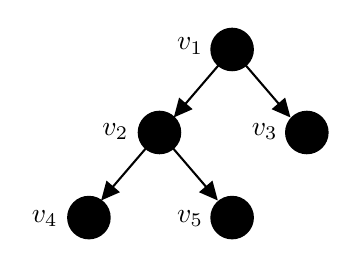
\begin{tikzpicture}[x=0.75pt,y=0.75pt,yscale=-1,xscale=1]
%uncomment if require: \path (0,151); %set diagram left start at 0, and has height of 151

%Straight Lines [id:da6269794272523825] 
\draw    (95,70) -- (121.15,100.47) ;
\draw [shift={(123.1,102.75)}, rotate = 229.37] [fill={rgb, 255:red, 0; green, 0; blue, 0 }  ][line width=0.08]  [draw opacity=0] (8.93,-4.29) -- (0,0) -- (8.93,4.29) -- cycle    ;
%Straight Lines [id:da986476888481959] 
\draw    (130,30) -- (156.15,60.47) ;
\draw [shift={(158.1,62.75)}, rotate = 229.37] [fill={rgb, 255:red, 0; green, 0; blue, 0 }  ][line width=0.08]  [draw opacity=0] (8.93,-4.29) -- (0,0) -- (8.93,4.29) -- cycle    ;
%Straight Lines [id:da44376792645731866] 
\draw    (95,70) -- (68.85,100.47) ;
\draw [shift={(66.9,102.75)}, rotate = 310.63] [fill={rgb, 255:red, 0; green, 0; blue, 0 }  ][line width=0.08]  [draw opacity=0] (8.93,-4.29) -- (0,0) -- (8.93,4.29) -- cycle    ;
%Straight Lines [id:da9694685289799305] 
\draw    (130,30) -- (103.85,60.47) ;
\draw [shift={(101.9,62.75)}, rotate = 310.63] [fill={rgb, 255:red, 0; green, 0; blue, 0 }  ][line width=0.08]  [draw opacity=0] (8.93,-4.29) -- (0,0) -- (8.93,4.29) -- cycle    ;
%Shape: Circle [id:dp9985907627673265] 
\draw  [fill={rgb, 255:red, 0; green, 0; blue, 0 }  ,fill opacity=1 ] (120,30) .. controls (120,24.48) and (124.48,20) .. (130,20) .. controls (135.52,20) and (140,24.48) .. (140,30) .. controls (140,35.52) and (135.52,40) .. (130,40) .. controls (124.48,40) and (120,35.52) .. (120,30) -- cycle ;
%Shape: Circle [id:dp9359075911835515] 
\draw  [fill={rgb, 255:red, 0; green, 0; blue, 0 }  ,fill opacity=1 ] (156,70) .. controls (156,64.48) and (160.48,60) .. (166,60) .. controls (171.52,60) and (176,64.48) .. (176,70) .. controls (176,75.52) and (171.52,80) .. (166,80) .. controls (160.48,80) and (156,75.52) .. (156,70) -- cycle ;
%Shape: Circle [id:dp3437213039907303] 
\draw  [fill={rgb, 255:red, 0; green, 0; blue, 0 }  ,fill opacity=1 ] (85,70) .. controls (85,64.48) and (89.48,60) .. (95,60) .. controls (100.52,60) and (105,64.48) .. (105,70) .. controls (105,75.52) and (100.52,80) .. (95,80) .. controls (89.48,80) and (85,75.52) .. (85,70) -- cycle ;
%Shape: Circle [id:dp8935393527337947] 
\draw  [fill={rgb, 255:red, 0; green, 0; blue, 0 }  ,fill opacity=1 ] (51,111) .. controls (51,105.48) and (55.48,101) .. (61,101) .. controls (66.52,101) and (71,105.48) .. (71,111) .. controls (71,116.52) and (66.52,121) .. (61,121) .. controls (55.48,121) and (51,116.52) .. (51,111) -- cycle ;
%Shape: Circle [id:dp3004114626227925] 
\draw  [fill={rgb, 255:red, 0; green, 0; blue, 0 }  ,fill opacity=1 ] (120,111) .. controls (120,105.48) and (124.48,101) .. (130,101) .. controls (135.52,101) and (140,105.48) .. (140,111) .. controls (140,116.52) and (135.52,121) .. (130,121) .. controls (124.48,121) and (120,116.52) .. (120,111) -- cycle ;

% Text Node
\draw (102,23) node [anchor=north west][inner sep=0.75pt]    {$v_{1}$};
% Text Node
\draw (66,64) node [anchor=north west][inner sep=0.75pt]    {$v_{2}$};
% Text Node
\draw (138,64) node [anchor=north west][inner sep=0.75pt]    {$v_{3}$};
% Text Node
\draw (102,106) node [anchor=north west][inner sep=0.75pt]    {$v_{5}$};
% Text Node
\draw (32,106) node [anchor=north west][inner sep=0.75pt]    {$v_{4}$};


\end{tikzpicture}}
        \caption{A Tree.}
        \label{fig:tree}
    \end{subfigure}
    % \begin{subfigure}[b]{0.32\linewidth}
    %     \centering
    %     \resizebox{.8\textwidth}{!}{\input{Figures/Chapter2/dpag.tex}}
    %     \caption{A DPAG.}
    %     \label{fig:dpag}
    % \end{subfigure}
    \caption{Special classes of graphs.}
\end{figure*}

\paragraph{Subgraphs and Induced Subgraphs} A \keyword{subgraph}
$H = \langle \Cal{V}_H, \Cal{E}_H \rangle$ of a graph $G$ is any graph for which $\Cal{V}_H \subseteq \Cal{V}_G$ and  $\Cal{E}_H \subseteq \Cal{E}_G$. If $\Cal{V}_H$ contains only vertices that are endpoints in $\Cal{E}_H$, the resulting subgraph is called \keyword{induced subgraph}, or the subgraph induced by $\Cal{V}_H$ in $G$. 

\subsection{Attributed Graphs} \label{sec:attr-graphs}
Real-world instances of graphs usually carry out other information besides structure, generally attached to their vertices or edges. As an example, consider the graph representation of a molecule, in which vertices are usually annotated with an atom type, and edges are annotated with a chemical bond type. Given a graph $G$ with $n$ vertices and $m$ edges, we define the associated graph with additional information content, and we call it an \keyword{attributed graph}, as a triplet:
$$\langle G, \psi, \zeta \rangle,$$
where $\psi: \Cal{V}_G \rightarrow \Real^d$ is a mapping from the space of vertices to a space of $d$-dimensional \emph{vertex features}, and $\zeta: \Cal{E}_G \rightarrow \Real^{e}$, is a mapping from the space of edges to a space of $e$-dimensional \emph{edge features}. The values of these features can be either discrete (in which case the features are called \emph{labels} and encoded as one-hot vectors) or continuous vectors. Sometimes, we omit to define $\psi$ and $\zeta$ explicitly, and provide the vertex and edge features directly as sets, \eg $\Vector{x}_G = \Set{\Elem{x}{v} \in \Real^d \mid v \in \Cal{V}_G}$ for the vertex features, and $\Vector{e}_G = \Set{\Elem{e}{u,v} \in \Real^e \mid (u, v) \in \Cal{E}_G}$ for the edge features.
If some ordering of the vertices and edges is assumed, we can represent equivalently $\psi$ as a matrix $\Matrix{x}_G \in \Real^{n \times d}$ where the $i$-th row contains the vertex features of the $i$-th vertex; analogously, we can define $\zeta$ as a matrix of edge features $\Matrix{E}_G \in \Real^{m \times e}$.

\subsection{Isomorphisms, Automorphisms, and Canonization} \label{sec:isomorphisms}
An \keyword{isomorphism} between two graphs $G$ and $H$ is a bijection $\phi: \Cal{V}_G \rightarrow \Cal{V}_H$ such that $(u,v) \in \Cal{E}_G$ if and only if $(\phi(u),\phi(v)) \in \Cal{E}_H$. Intuitively, graph isomorphism formalizes the notion of \emph{structural equivalence} between graphs, in the sense that two isomorphic graphs are structurally equivalent, regardless of the information they contain. Figure \ref{fig:isomorphism} shows two isomorphic graphs and their corresponding $\phi$ bijection. An \keyword{automorphism} $\pi: \Cal{V}_G \rightarrow \Cal{V}_G$ is an isomorphism between $G$ and itself. Since $\pi$ is essentially a permutation of the vertex set, it follows that a graph always has at most $n!$ possible automorphisms. Intuitively, and similarly to graph isomorphism, graph automorphisms convey the notion that the structure of a graph is invariant to permutation of the vertices and edges. An automorphism $\pi$ on an example graph is shown
in Figure \ref{fig:automorphism}. Related to isomorphisms and automorphisms is the problem of \keyword{graph canonization}, where a canonical ordering (or form) of the graph vertices is sought, such that every graph $H$ isomorph to a given graph $G$ has the same canonical form. As we shall see, (approximate) graph canonization plays a role in the usage of graph within practical contexts; conversely, many techniques described in this work try to avoid representing graphs in canonical form, in favor of permutation-invariant representations.

\begin{figure*}
    \begin{subfigure}[b]{0.48\linewidth}
        \centering
        \resizebox{.9\textwidth}{!}{

\tikzset{every picture/.style={line width=0.75pt}} %set default line width to 0.75pt

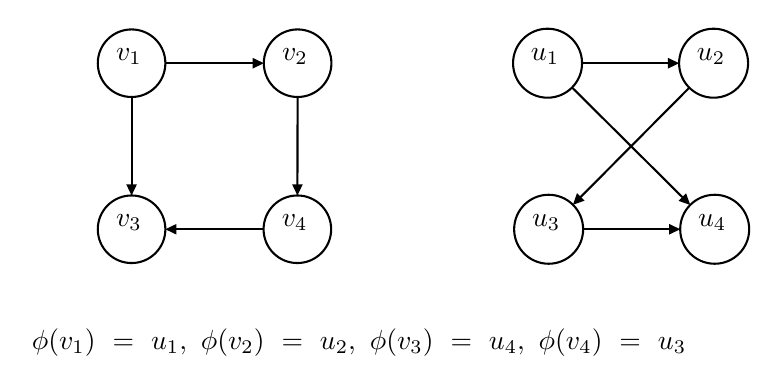
\begin{tikzpicture}[x=0.75pt,y=0.75pt,yscale=-1,xscale=1]
%uncomment if require: \path (0,184); %set diagram left start at 0, and has height of 184


% Text Node
\draw (5,157.4) node [anchor=north west][inner sep=0.75pt]    {$\phi ( v_{1}) \ =\ u_{1} ,\ \phi ( v_{2}) \ =\ u_{2} ,\ \phi ( v_{3}) \ =\ u_{4} ,\ \phi ( v_{4}) \ =\ u_{3}$};
% Text Node
\draw    (335.5, 111) circle [x radius= 16.62, y radius= 16.62]   ;
\draw (326,102.4) node [anchor=north west][inner sep=0.75pt]    {$u_{4}$};
% Text Node
\draw    (255.5, 111) circle [x radius= 16.62, y radius= 16.62]   ;
\draw (246,102.4) node [anchor=north west][inner sep=0.75pt]    {$u_{3}$};
% Text Node
\draw    (54.56, 31) circle [x radius= 16.28, y radius= 16.28]   ;
\draw (45.56,22.4) node [anchor=north west][inner sep=0.75pt]    {$v_{1}$};
% Text Node
\draw    (54.56, 111) circle [x radius= 16.28, y radius= 16.28]   ;
\draw (45.56,102.4) node [anchor=north west][inner sep=0.75pt]    {$v_{3}$};
% Text Node
\draw    (134.56, 31) circle [x radius= 16.28, y radius= 16.28]   ;
\draw (125.56,22.4) node [anchor=north west][inner sep=0.75pt]    {$v_{2}$};
% Text Node
\draw    (134.44, 111) circle [x radius= 16.28, y radius= 16.28]   ;
\draw (125.44,102.4) node [anchor=north west][inner sep=0.75pt]    {$v_{4}$};
% Text Node
\draw    (254.98, 31) circle [x radius= 16.62, y radius= 16.62]   ;
\draw (245.48,22.4) node [anchor=north west][inner sep=0.75pt]    {$u_{1}$};
% Text Node
\draw    (334.98, 31) circle [x radius= 16.62, y radius= 16.62]   ;
\draw (325.48,22.4) node [anchor=north west][inner sep=0.75pt]    {$u_{2}$};
% Connection
\draw    (272.12,111) -- (315.88,111) ;
\draw [shift={(318.88,111)}, rotate = 180] [fill={rgb, 255:red, 0; green, 0; blue, 0 }  ][line width=0.08]  [draw opacity=0] (5.36,-2.57) -- (0,0) -- (5.36,2.57) -- cycle    ;
% Connection
\draw    (54.56,47.28) -- (54.56,91.72) ;
\draw [shift={(54.56,94.72)}, rotate = 270] [fill={rgb, 255:red, 0; green, 0; blue, 0 }  ][line width=0.08]  [draw opacity=0] (5.36,-2.57) -- (0,0) -- (5.36,2.57) -- cycle    ;
% Connection
\draw    (70.84,31) -- (115.28,31) ;
\draw [shift={(118.28,31)}, rotate = 180] [fill={rgb, 255:red, 0; green, 0; blue, 0 }  ][line width=0.08]  [draw opacity=0] (5.36,-2.57) -- (0,0) -- (5.36,2.57) -- cycle    ;
% Connection
\draw    (134.54,47.28) -- (134.47,91.72) ;
\draw [shift={(134.46,94.72)}, rotate = 270.09000000000003] [fill={rgb, 255:red, 0; green, 0; blue, 0 }  ][line width=0.08]  [draw opacity=0] (5.36,-2.57) -- (0,0) -- (5.36,2.57) -- cycle    ;
% Connection
\draw    (118.16,111) -- (73.84,111) ;
\draw [shift={(70.84,111)}, rotate = 360] [fill={rgb, 255:red, 0; green, 0; blue, 0 }  ][line width=0.08]  [draw opacity=0] (5.36,-2.57) -- (0,0) -- (5.36,2.57) -- cycle    ;
% Connection
\draw    (271.6,31) -- (315.36,31) ;
\draw [shift={(318.36,31)}, rotate = 540] [fill={rgb, 255:red, 0; green, 0; blue, 0 }  ][line width=0.08]  [draw opacity=0] (5.36,-2.57) -- (0,0) -- (5.36,2.57) -- cycle    ;
% Connection
\draw    (266.77,42.71) -- (321.58,97.17) ;
\draw [shift={(323.71,99.29)}, rotate = 224.81] [fill={rgb, 255:red, 0; green, 0; blue, 0 }  ][line width=0.08]  [draw opacity=0] (5.36,-2.57) -- (0,0) -- (5.36,2.57) -- cycle    ;
% Connection
\draw    (323.27,42.79) -- (269.33,97.08) ;
\draw [shift={(267.21,99.21)}, rotate = 314.81] [fill={rgb, 255:red, 0; green, 0; blue, 0 }  ][line width=0.08]  [draw opacity=0] (5.36,-2.57) -- (0,0) -- (5.36,2.57) -- cycle    ;

\end{tikzpicture}}
        \caption{Isomorphism.}
        \label{fig:isomorphism}
    \end{subfigure}
    \begin{subfigure}[b]{0.48\linewidth}
        \centering
        \resizebox{.9\textwidth}{!}{

\tikzset{every picture/.style={line width=0.75pt}} %set default line width to 0.75pt

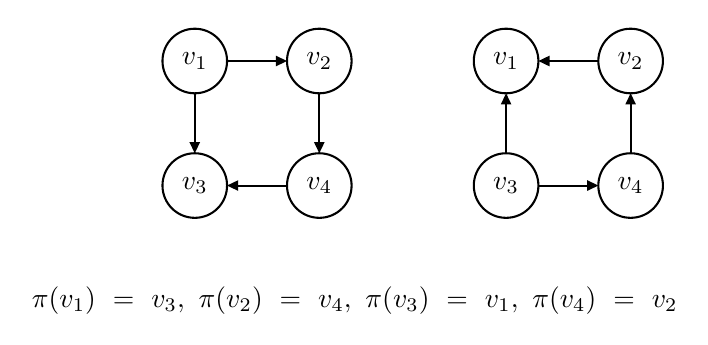
\begin{tikzpicture}[x=0.75pt,y=0.75pt,yscale=-1,xscale=1]
%uncomment if require: \path (0,194); %set diagram left start at 0, and has height of 194


% Text Node
\draw (210,157.4) node [anchor=north west][inner sep=0.75pt]    {$\pi ( v_{1}) \ =\ v_{3} ,\ \pi ( v_{2}) \ =\ v_{4} ,\ \pi ( v_{3}) \ =\ v_{1} ,\ \pi ( v_{4}) \ =\ v_{2}$};
% Text Node
\draw    (290, 50) circle [x radius= 15.56, y radius= 15.56]   ;
\draw (290,50) node   [align=left] {\begin{minipage}[lt]{13.600000000000001pt}\setlength\topsep{0pt}
\begin{center}
$\displaystyle v_{1}$
\end{center}

\end{minipage}};
% Text Node
\draw    (290, 110) circle [x radius= 15.56, y radius= 15.56]   ;
\draw (290,110) node   [align=left] {\begin{minipage}[lt]{13.600000000000001pt}\setlength\topsep{0pt}
\begin{center}
$\displaystyle v_{3}$
\end{center}

\end{minipage}};
% Text Node
\draw    (350, 110) circle [x radius= 15.56, y radius= 15.56]   ;
\draw (350,110) node   [align=left] {\begin{minipage}[lt]{13.600000000000001pt}\setlength\topsep{0pt}
\begin{center}
$\displaystyle v_{4}$
\end{center}

\end{minipage}};
% Text Node
\draw    (350, 50) circle [x radius= 15.56, y radius= 15.56]   ;
\draw (350,50) node   [align=left] {\begin{minipage}[lt]{13.600000000000001pt}\setlength\topsep{0pt}
\begin{center}
$\displaystyle v_{2}$
\end{center}

\end{minipage}};
% Text Node
\draw    (440, 50) circle [x radius= 15.56, y radius= 15.56]   ;
\draw (440,50) node   [align=left] {\begin{minipage}[lt]{13.600000000000001pt}\setlength\topsep{0pt}
\begin{center}
$\displaystyle v_{1}$
\end{center}

\end{minipage}};
% Text Node
\draw    (440, 110) circle [x radius= 15.56, y radius= 15.56]   ;
\draw (440,110) node   [align=left] {\begin{minipage}[lt]{13.600000000000001pt}\setlength\topsep{0pt}
\begin{center}
$\displaystyle v_{3}$
\end{center}

\end{minipage}};
% Text Node
\draw    (500, 110) circle [x radius= 15.56, y radius= 15.56]   ;
\draw (500,110) node   [align=left] {\begin{minipage}[lt]{13.600000000000001pt}\setlength\topsep{0pt}
\begin{center}
$\displaystyle v_{4}$
\end{center}

\end{minipage}};
% Text Node
\draw    (500, 50) circle [x radius= 15.56, y radius= 15.56]   ;
\draw (500,50) node   [align=left] {\begin{minipage}[lt]{13.600000000000001pt}\setlength\topsep{0pt}
\begin{center}
$\displaystyle v_{2}$
\end{center}

\end{minipage}};
% Connection
\draw    (305.56,50) -- (331.44,50) ;
\draw [shift={(334.44,50)}, rotate = 180] [fill={rgb, 255:red, 0; green, 0; blue, 0 }  ][line width=0.08]  [draw opacity=0] (5.36,-2.57) -- (0,0) -- (5.36,2.57) -- cycle    ;
% Connection
\draw    (350,65.56) -- (350,91.44) ;
\draw [shift={(350,94.44)}, rotate = 270] [fill={rgb, 255:red, 0; green, 0; blue, 0 }  ][line width=0.08]  [draw opacity=0] (5.36,-2.57) -- (0,0) -- (5.36,2.57) -- cycle    ;
% Connection
\draw    (334.44,110) -- (308.56,110) ;
\draw [shift={(305.56,110)}, rotate = 360] [fill={rgb, 255:red, 0; green, 0; blue, 0 }  ][line width=0.08]  [draw opacity=0] (5.36,-2.57) -- (0,0) -- (5.36,2.57) -- cycle    ;
% Connection
\draw    (290,65.56) -- (290,91.44) ;
\draw [shift={(290,94.44)}, rotate = 270] [fill={rgb, 255:red, 0; green, 0; blue, 0 }  ][line width=0.08]  [draw opacity=0] (5.36,-2.57) -- (0,0) -- (5.36,2.57) -- cycle    ;
% Connection
\draw    (484.44,50) -- (458.56,50) ;
\draw [shift={(455.56,50)}, rotate = 360] [fill={rgb, 255:red, 0; green, 0; blue, 0 }  ][line width=0.08]  [draw opacity=0] (5.36,-2.57) -- (0,0) -- (5.36,2.57) -- cycle    ;
% Connection
\draw    (500,94.44) -- (500,68.56) ;
\draw [shift={(500,65.56)}, rotate = 450] [fill={rgb, 255:red, 0; green, 0; blue, 0 }  ][line width=0.08]  [draw opacity=0] (5.36,-2.57) -- (0,0) -- (5.36,2.57) -- cycle    ;
% Connection
\draw    (455.56,110) -- (481.44,110) ;
\draw [shift={(484.44,110)}, rotate = 180] [fill={rgb, 255:red, 0; green, 0; blue, 0 }  ][line width=0.08]  [draw opacity=0] (5.36,-2.57) -- (0,0) -- (5.36,2.57) -- cycle    ;
% Connection
\draw    (440,94.44) -- (440,68.56) ;
\draw [shift={(440,65.56)}, rotate = 450] [fill={rgb, 255:red, 0; green, 0; blue, 0 }  ][line width=0.08]  [draw opacity=0] (5.36,-2.57) -- (0,0) -- (5.36,2.57) -- cycle    ;

\end{tikzpicture}}
        \caption{Automorphism.}
        \label{fig:automorphism}
    \end{subfigure}
    \caption{An example of isomorphism and automorphism.}
\end{figure*}

\subsection{Graphs as Matrices} \label{sec:adj-matrix}
One compact way to represent the structure of a graph is through its  \keyword{adjacency matrix}. Given a graph $G$ with $n$ vertices and $m$ edges, the entries of its corresponding  adjacency matrix $\Matrix{A} \in \mathbb{R}^{n \times n}$ are defined as follows:
\[
\Matrix{A}_{ij} =
    \begin{cases}
        1  & \text{if } (v_i, v_j) \in \Cal{E}_G \\
        0  & \text{otherwise.}
    \end{cases}
\]
Note that the diagonal entries $\Matrix{A}_{ii}$ of the adjacency matrix specify the presence  (or absence) of self-loops. Another interesting property of the adjacency matrix is that  it is symmetric for undirected graphs, which implies $\Matrix{A}_{ij} = \Matrix{A}_{ji},$ $\forall i, j = 1, \ldots, n$. Adjacency matrices make some calculations of graph properties particularly convenient: for example, the in-degree and out-degree of a vertex $v_j \in G$
can be obtained by performing row-wise and column-wise sums on $\Matrix{A}$:
$$
\Fun{degree}_{in}(v_j) = \sum_{i=1}^n \Matrix{A}_{ji} \quad \quad \Fun{degree}_{out}(v_j) = \sum_{i=1}^n \Matrix{A}_{ij}.
$$
Adjacency matrices are also useful to understand concepts such as graph automorphisms: in fact, an automorphism of $G$ corresponds to a permutation of the columns or rows of the adjacency matrix (but not both). Other useful matrices to represent properties graphs are the \emph{Laplacian matrix} $\Matrix{L} \in \Real^{n \times n} = \Matrix{D} - \Matrix{A}$, and the \emph{symmetric normalized Laplacian matrix} $\Matrix{\tilde{L}} \in \Real^{n \times n} = \Matrix{I} - \Matrix{D}^{-\frac{1}{2}}\Matrix{A}\Matrix{D}^{-\frac{1}{2}}$. In both definitions, the matrix  $\Matrix{D} \in \Real^{n \times n}$ is the \emph{degree matrix}, where all entries are zero except the diagonal entries, for which $\Matrix{D}_{ii} = \Fun{degree}(v_i)$. These matrices provide information about the graph connectivity through their eigenvalues and eigenvectors.

\section{The Adaptive Processing of Structured Data}
The processing of structured data for learning purposes is carried out by a \keyword{structural transduction}, namely a function $\Transduction: \Cal{x} \shortrightarrow \Cal{y}$ where $\Cal{X}$ and $\Cal{Y}$ are structured domains. When the structural transduction is implemented by a (deep) \gls{nn}, it is \emph{adaptive}, \ie it is learned from data. A structural transduction can be decomposed as $\Transduction = \Transduction_{\Fun{enc}} \circ \Transduction_{\Fun{out}}$, where:
\begin{itemize}
    \item $\Transduction_{\Fun{enc}}$ is called \emph{encoding function} or \emph{state transition function} that is applied separately to each element of the structure. The output of the encoding function is a structure isomorphic to that in input, where the elements are now \keyword{state vectors}. Intuitively, a state vector encodes the information of the element and of the elements it depends on;
    \item $\Transduction_{\Fun{out}}$ is called \emph{output function}, which computes an output from the state vectors.
\end{itemize}
The output function of the structural transduction is task-dependent. Considering a supervised setting and a generic graph dataset $\Data_n$ consisting of $n$ training pairs, we distinguish two learning problems:
\begin{itemize}
    \item in \emph{structure-to-structure} tasks, the dataset has the form $\Data_n = \Set{(\Vector{x}_G^{(i)}, \Vector{y}_H^{(i)})}_{i=1}^n$, and the output function maps each element of the structured datum to an output. More specifically, a training pair is defined as $\Cal{S} = (\Vector{x}_G, \Vector{y}_H)$, where $\Vector{x}_G = \Set{\Elem{x}{v} \mid v \in \Cal{V}_G}$ and $\Vector{y}_H = \Set{\Elem{y}{\phi(v)} \mid v \in \Cal{V}_{G}}$, with $G$ isomorphic to $H$ under a bijection $\phi$. The \gls{mle} objective function minimized in these tasks is the following:
    $$\argmin_{\Param} \frac{1}{n} \sum_{\Cal{S} \in \Data_n} - \log p_{\Param}(\Vector{y}_H \given \Vector{x}_G) = \frac{1}{n}\sum_{\Cal{S} \in \Data_n} \sum_{v \in \Cal{V}_G} - \log p_{\Param}(\Elem{y}{\phi(v)} \given \Elem{x}{v}),$$
    where $p_{\Param}$ is a neural network with parameters $\Param$ that learns an approximation of the true conditional.
    \item in \emph{structure-to-element} tasks, the dataset has the form $\Data_n = \Set{(\Vector{x}_G^{(i)}, \Vector{y}^{(i)})}_{i=1}^n$, and the output function maps the whole structure to a single output vector (or scalar). More specifically, a training pair is defined as $\Cal{S} = (\Vector{x}_G, \Vector{y})$, where $\Vector{y} \in \Real^y$. The \gls{mle} objective function minimized in these tasks is the following:
    $$\argmin_{\Param} \frac{1}{n} \sum_{\Cal{S} \in \Data_n} - \log p_{\Param}(\Vector{y} \given \Vector{x}_G).$$
    To learn structure-to-element tasks, the output function must compress the states of each element of the structure into a global output vector representing the entire structure, which is compared to the target $\Vector{y}$. To do so, there are several strategies; in general, one could pick a single state vector as a representative for the whole structure, or compute a summary of the entire structure using all the available state vectors. The function that implements the latter strategy is usually termed \keyword{readout}. 
\end{itemize}

As anticipated, one important issue that structural transductions need to address is how to deal with variable-sized inputs. The solution is to apply the same state transition function (that is, with the same adaptive parameters) \emph{locally} to every element in the structure, rather than to apply it one time to the overall structure. This process is similar to the localized processing of images performed by \glspl{cnn} \cite{?}, which works by considering a single pixel at a time, and combining it with some finite set of nearby pixels. This local property of the structural transduction is often referred to as \emph{stationarity}. An interesting byproduct of using stationary transductions is that they require a smaller number of parameters with respect to non-stationary ones, since the network weights are shared across the structure. At the same time, using stationary transductions also requires additional mechanisms to learn from the global structure of the datum (such as readouts in the case of structure-to-element tasks), rather than only locally.

In the following sections, we present three specific \gls{nn} architectures that implement transductions over structured data: recurrent neural networks, which process data represented as sequences; recursive neural networks, which process hierarchical data such as trees; and deep graph networks, which process general graphs.

\section{Recurrent Neural Networks}\label{sec:rnns}
A \gls{rnn} is a \gls{nn} architecture able to process sequences. Let $S$ be a sequence of length $m$ whose set of elements is $\Cal{V}_S = (v_1, v_2, \ldots, v_m)$, and let $S_{\Vector{x}} = \Seq{\Elem{x}{1}, \Elem{x}{2}, \ldots, \Elem{x}{m}}$ be its element features. Here, we slightly abuse the notation $\Elem{h}{v_t}$ in favor of $\Elem{h}{t}$ since sequence elements are ordered. The state transition function of a \gls{rnn}, applied locally to each sequence element, has the following general form:
\begin{align*}
    \Elem{h}{t} &= \Transduction_{\Fun{enc}}(\Elem{x}{t}, \Elem{h}{t-1}),
\end{align*}
where $\Elem{h}{t} \in \Real^h$ is a state vector, also known as \keyword{hidden state}. The calculation of the hidden state performed by the state transition function $\Transduction_{\Fun{enc}}$ is \emph{recursive}: to compute a hidden state for the $t$-th element of the sequence, the hidden state of the previous element must be known in advance. Thus, the state computation is a sequential process, where the input sequence is traversed in order one element at a time, and the hidden state is updated as a function of the current sequence element and the hidden state at the previous step. To avoid infinite recursion, the hidden state is initialized with a vector $\Elem{h}{0}$. As the sequence is traversed, the hidden state maintains a \emph{memory} of the past elements of the sequence. The presence of a memory mechanism makes \glspl{rnn} very powerful: in fact, it has been proved that finite-size \glspl{rnn} can compute any function computable with a Turing machine \cite{?}. As with \glspl{cnn}, the development of \glspl{rnn} started in the early '90s, and they have recently been rediscovered within the \gls{dl} framework after their success, especially in \gls{nlp}-related tasks.

\subsection{Training}
Given a sequence $S$ with features $S_{\Vector{x}}$, the original implementation of the state transition function of a \gls{rnn} is defined as follows\footnote{For the rest of this chapter, biases are omitted for readability.}:
\begin{align*}
    \Elem{h}{t} &= \Fun{tanh}\Paren{\Matrix{W}^{\Transpose}\Elem{x}{t} + \Matrix{U}^{\Transpose}\Elem{h}{t-1}},\; \forall t=1, \ldots, m.
\end{align*}
The above is also called \keyword{recurrent layer}. The weight matrices $\Matrix{W} \in \Real^{d \times h}$ and $\Matrix{U} \in \Real^{h \times h}$, are shared among the sequence elements according to the stationarity property. For this reason, it is often said that the network is \emph{unrolled} over the sequence. In structure-to-structure tasks, once the states of the elements are calculated, an element-wise output is computed as:
\begin{align*}
    \Elem{o}{t} = g_{\mathrm{out}}(\Elem{h}{t}),\; \forall t=1, \ldots, m,
\end{align*}
where $g_{\mathrm{out}}$ can be any neural network such as one simple output layer or a more complex downstream network. Similarly, in structure-to-element tasks, a single output is computed from the last hidden state of the sequence:
\begin{align*}
    \Vector{o} = g_{\mathrm{out}}(\Elem{h}{m}).
\end{align*}
Figure \ref{fig:rnn-unfold} shows a \gls{rnn} in compact form, as well as unrolled over a sequence of length $m$ for a structure-to-structure task. The error of the network during training is computed by comparing the output of the network for each sequence element $\Elem{o}{t}$ to the corresponding sequence element $\Elem{y}{t}$ in the target sequence with the loss function $\Loss$, which is summed up over all the elements in the sequence. Notice that it is possible to stack multiple recurrent layers and create deep \glspl{rnn} by feeding the hidden state produced the recurrent layer to a subsequent recurrent layer, other than to the next step of the recurrence. In this cases, the output is computed after the last recurrent layer.
\begin{figure*}[h!]
    \begin{subfigure}[b]{0.4\linewidth}
        \centering
        \resizebox{.6\textwidth}{!}{

\tikzset{every picture/.style={line width=0.75pt}} %set default line width to 0.75pt

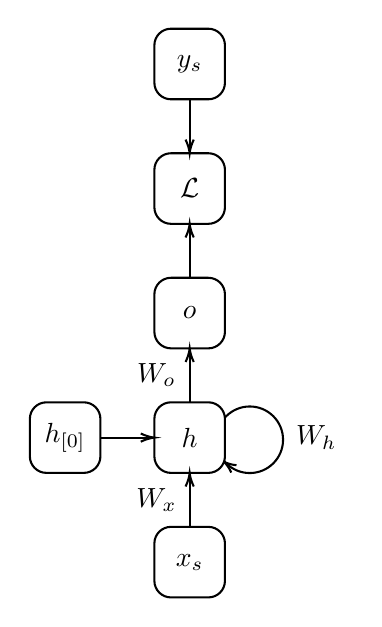
\begin{tikzpicture}[x=0.75pt,y=0.75pt,yscale=-1,xscale=1]
%uncomment if require: \path (0,300); %set diagram left start at 0, and has height of 300

%Shape: Circle [id:dp23367042930106008]
\draw   (107.92,216.04) .. controls (107.92,207.18) and (115.1,200) .. (123.96,200) .. controls (132.82,200) and (140,207.18) .. (140,216.04) .. controls (140,224.9) and (132.82,232.08) .. (123.96,232.08) .. controls (115.1,232.08) and (107.92,224.9) .. (107.92,216.04) -- cycle ;
\draw   (115.05,231.82) .. controls (114.1,229.66) and (112.86,227.9) .. (111.36,226.53) .. controls (113.14,227.51) and (115.22,228.09) .. (117.57,228.29) ;

% Text Node
\draw    (78,266) .. controls (78,261.58) and (81.58,258) .. (86,258) -- (104,258) .. controls (108.42,258) and (112,261.58) .. (112,266) -- (112,284) .. controls (112,288.42) and (108.42,292) .. (104,292) -- (86,292) .. controls (81.58,292) and (78,288.42) .. (78,284) -- cycle  ;
\draw (95,275) node   [align=left] {\begin{minipage}[lt]{20.400000000000002pt}\setlength\topsep{0pt}
\begin{center}
$\displaystyle \boldsymbol{x}_{s}$
\end{center}

\end{minipage}};
% Text Node
\draw  [fill={rgb, 255:red, 255; green, 255; blue, 255 }  ,fill opacity=1 ]  (78,206) .. controls (78,201.58) and (81.58,198) .. (86,198) -- (104,198) .. controls (108.42,198) and (112,201.58) .. (112,206) -- (112,224) .. controls (112,228.42) and (108.42,232) .. (104,232) -- (86,232) .. controls (81.58,232) and (78,228.42) .. (78,224) -- cycle  ;
\draw (95,215) node   [align=left] {\begin{minipage}[lt]{20.400000000000002pt}\setlength\topsep{0pt}
\begin{center}
$\displaystyle \boldsymbol{h}$
\end{center}

\end{minipage}};
% Text Node
\draw    (18,206) .. controls (18,201.58) and (21.58,198) .. (26,198) -- (44,198) .. controls (48.42,198) and (52,201.58) .. (52,206) -- (52,224) .. controls (52,228.42) and (48.42,232) .. (44,232) -- (26,232) .. controls (21.58,232) and (18,228.42) .. (18,224) -- cycle  ;
\draw (35,215) node   [align=left] {\begin{minipage}[lt]{20.400000000000002pt}\setlength\topsep{0pt}
\begin{center}
$\displaystyle \boldsymbol{h}_{[ 0]}$
\end{center}

\end{minipage}};
% Text Node
\draw    (78,146) .. controls (78,141.58) and (81.58,138) .. (86,138) -- (104,138) .. controls (108.42,138) and (112,141.58) .. (112,146) -- (112,164) .. controls (112,168.42) and (108.42,172) .. (104,172) -- (86,172) .. controls (81.58,172) and (78,168.42) .. (78,164) -- cycle  ;
\draw (95,155) node   [align=left] {\begin{minipage}[lt]{20.400000000000002pt}\setlength\topsep{0pt}
\begin{center}
$\displaystyle \boldsymbol{o}$
\end{center}

\end{minipage}};
% Text Node
\draw    (78,86) .. controls (78,81.58) and (81.58,78) .. (86,78) -- (104,78) .. controls (108.42,78) and (112,81.58) .. (112,86) -- (112,104) .. controls (112,108.42) and (108.42,112) .. (104,112) -- (86,112) .. controls (81.58,112) and (78,108.42) .. (78,104) -- cycle  ;
\draw (95,95) node   [align=left] {\begin{minipage}[lt]{20.400000000000002pt}\setlength\topsep{0pt}
\begin{center}
$\displaystyle \mathcal{L}$
\end{center}

\end{minipage}};
% Text Node
\draw    (78,26) .. controls (78,21.58) and (81.58,18) .. (86,18) -- (104,18) .. controls (108.42,18) and (112,21.58) .. (112,26) -- (112,44) .. controls (112,48.42) and (108.42,52) .. (104,52) -- (86,52) .. controls (81.58,52) and (78,48.42) .. (78,44) -- cycle  ;
\draw (95,35) node   [align=left] {\begin{minipage}[lt]{20.400000000000002pt}\setlength\topsep{0pt}
\begin{center}
$\displaystyle \boldsymbol{y}_{s}$
\end{center}

\end{minipage}};
% Text Node
\draw (156,215) node   [align=left] {\begin{minipage}[lt]{20.400000000000002pt}\setlength\topsep{0pt}
\begin{center}
$\displaystyle \boldsymbol{W}_{h}$
\end{center}

\end{minipage}};
% Text Node
\draw (79,245) node   [align=left] {\begin{minipage}[lt]{20.400000000000002pt}\setlength\topsep{0pt}
\begin{center}
$\displaystyle \boldsymbol{W}_{x}$
\end{center}

\end{minipage}};
% Text Node
\draw (79,185) node   [align=left] {\begin{minipage}[lt]{20.400000000000002pt}\setlength\topsep{0pt}
\begin{center}
$\displaystyle \boldsymbol{W}_{o}$
\end{center}

\end{minipage}};
% Connection
\draw    (95,258) -- (95,234) ;
\draw [shift={(95,232)}, rotate = 450] [color={rgb, 255:red, 0; green, 0; blue, 0 }  ][line width=0.75]    (6.56,-1.97) .. controls (4.17,-0.84) and (1.99,-0.18) .. (0,0) .. controls (1.99,0.18) and (4.17,0.84) .. (6.56,1.97)   ;
% Connection
\draw    (52,215) -- (76,215) ;
\draw [shift={(78,215)}, rotate = 180] [color={rgb, 255:red, 0; green, 0; blue, 0 }  ][line width=0.75]    (6.56,-1.97) .. controls (4.17,-0.84) and (1.99,-0.18) .. (0,0) .. controls (1.99,0.18) and (4.17,0.84) .. (6.56,1.97)   ;
% Connection
\draw    (95,198) -- (95,174) ;
\draw [shift={(95,172)}, rotate = 450] [color={rgb, 255:red, 0; green, 0; blue, 0 }  ][line width=0.75]    (6.56,-1.97) .. controls (4.17,-0.84) and (1.99,-0.18) .. (0,0) .. controls (1.99,0.18) and (4.17,0.84) .. (6.56,1.97)   ;
% Connection
\draw    (95,138) -- (95,114) ;
\draw [shift={(95,112)}, rotate = 450] [color={rgb, 255:red, 0; green, 0; blue, 0 }  ][line width=0.75]    (6.56,-1.97) .. controls (4.17,-0.84) and (1.99,-0.18) .. (0,0) .. controls (1.99,0.18) and (4.17,0.84) .. (6.56,1.97)   ;
% Connection
\draw    (95,52) -- (95,76) ;
\draw [shift={(95,78)}, rotate = 270] [color={rgb, 255:red, 0; green, 0; blue, 0 }  ][line width=0.75]    (6.56,-1.97) .. controls (4.17,-0.84) and (1.99,-0.18) .. (0,0) .. controls (1.99,0.18) and (4.17,0.84) .. (6.56,1.97)   ;

\end{tikzpicture}}
        \caption{}
        \label{fig:rnn}
    \end{subfigure}
    \begin{subfigure}[b]{0.59\linewidth}
        \centering
        \resizebox{.8\textwidth}{!}{

\tikzset{every picture/.style={line width=0.75pt}} %set default line width to 0.75pt

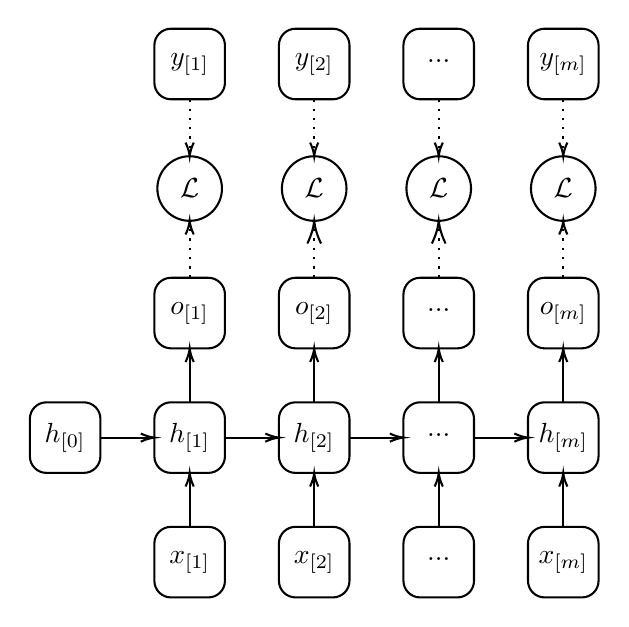
\begin{tikzpicture}[x=0.75pt,y=0.75pt,yscale=-1,xscale=1]
%uncomment if require: \path (0,300); %set diagram left start at 0, and has height of 300


% Text Node
\draw    (268,261) .. controls (268,256.58) and (271.58,253) .. (276,253) -- (294,253) .. controls (298.42,253) and (302,256.58) .. (302,261) -- (302,279) .. controls (302,283.42) and (298.42,287) .. (294,287) -- (276,287) .. controls (271.58,287) and (268,283.42) .. (268,279) -- cycle  ;
\draw (285,270) node   [align=left] {\begin{minipage}[lt]{20.400000000000002pt}\setlength\topsep{0pt}
\begin{center}
$\displaystyle \boldsymbol{x}_{[ 1]}$
\end{center}

\end{minipage}};
% Text Node
\draw  [fill={rgb, 255:red, 255; green, 255; blue, 255 }  ,fill opacity=1 ]  (268,201) .. controls (268,196.58) and (271.58,193) .. (276,193) -- (294,193) .. controls (298.42,193) and (302,196.58) .. (302,201) -- (302,219) .. controls (302,223.42) and (298.42,227) .. (294,227) -- (276,227) .. controls (271.58,227) and (268,223.42) .. (268,219) -- cycle  ;
\draw (285,210) node   [align=left] {\begin{minipage}[lt]{20.400000000000002pt}\setlength\topsep{0pt}
\begin{center}
$\displaystyle \boldsymbol{h}_{[ 1]}$
\end{center}

\end{minipage}};
% Text Node
\draw    (208,201) .. controls (208,196.58) and (211.58,193) .. (216,193) -- (234,193) .. controls (238.42,193) and (242,196.58) .. (242,201) -- (242,219) .. controls (242,223.42) and (238.42,227) .. (234,227) -- (216,227) .. controls (211.58,227) and (208,223.42) .. (208,219) -- cycle  ;
\draw (225,210) node   [align=left] {\begin{minipage}[lt]{20.400000000000002pt}\setlength\topsep{0pt}
\begin{center}
$\displaystyle \boldsymbol{h}_{[ 0]}$
\end{center}

\end{minipage}};
% Text Node
\draw    (268,141) .. controls (268,136.58) and (271.58,133) .. (276,133) -- (294,133) .. controls (298.42,133) and (302,136.58) .. (302,141) -- (302,159) .. controls (302,163.42) and (298.42,167) .. (294,167) -- (276,167) .. controls (271.58,167) and (268,163.42) .. (268,159) -- cycle  ;
\draw (285,150) node   [align=left] {\begin{minipage}[lt]{20.400000000000002pt}\setlength\topsep{0pt}
\begin{center}
$\displaystyle \boldsymbol{o}_{[ 1]}$
\end{center}

\end{minipage}};
% Text Node
\draw    (268,21) .. controls (268,16.58) and (271.58,13) .. (276,13) -- (294,13) .. controls (298.42,13) and (302,16.58) .. (302,21) -- (302,39) .. controls (302,43.42) and (298.42,47) .. (294,47) -- (276,47) .. controls (271.58,47) and (268,43.42) .. (268,39) -- cycle  ;
\draw (285,30) node   [align=left] {\begin{minipage}[lt]{20.400000000000002pt}\setlength\topsep{0pt}
\begin{center}
$\displaystyle \boldsymbol{y}_{[ 1]}$
\end{center}

\end{minipage}};
% Text Node
\draw    (328,261) .. controls (328,256.58) and (331.58,253) .. (336,253) -- (354,253) .. controls (358.42,253) and (362,256.58) .. (362,261) -- (362,279) .. controls (362,283.42) and (358.42,287) .. (354,287) -- (336,287) .. controls (331.58,287) and (328,283.42) .. (328,279) -- cycle  ;
\draw (345,270) node   [align=left] {\begin{minipage}[lt]{20.400000000000002pt}\setlength\topsep{0pt}
\begin{center}
$\displaystyle \boldsymbol{x}_{[ 2]}$
\end{center}

\end{minipage}};
% Text Node
\draw  [fill={rgb, 255:red, 255; green, 255; blue, 255 }  ,fill opacity=1 ]  (328,201) .. controls (328,196.58) and (331.58,193) .. (336,193) -- (354,193) .. controls (358.42,193) and (362,196.58) .. (362,201) -- (362,219) .. controls (362,223.42) and (358.42,227) .. (354,227) -- (336,227) .. controls (331.58,227) and (328,223.42) .. (328,219) -- cycle  ;
\draw (345,210) node   [align=left] {\begin{minipage}[lt]{20.400000000000002pt}\setlength\topsep{0pt}
\begin{center}
$\displaystyle \boldsymbol{h}_{[ 2]}$
\end{center}

\end{minipage}};
% Text Node
\draw    (328,141) .. controls (328,136.58) and (331.58,133) .. (336,133) -- (354,133) .. controls (358.42,133) and (362,136.58) .. (362,141) -- (362,159) .. controls (362,163.42) and (358.42,167) .. (354,167) -- (336,167) .. controls (331.58,167) and (328,163.42) .. (328,159) -- cycle  ;
\draw (345,150) node   [align=left] {\begin{minipage}[lt]{20.400000000000002pt}\setlength\topsep{0pt}
\begin{center}
$\displaystyle \boldsymbol{o}_{[ 2]}$
\end{center}

\end{minipage}};
% Text Node
\draw    (328,21) .. controls (328,16.58) and (331.58,13) .. (336,13) -- (354,13) .. controls (358.42,13) and (362,16.58) .. (362,21) -- (362,39) .. controls (362,43.42) and (358.42,47) .. (354,47) -- (336,47) .. controls (331.58,47) and (328,43.42) .. (328,39) -- cycle  ;
\draw (345,30) node   [align=left] {\begin{minipage}[lt]{20.400000000000002pt}\setlength\topsep{0pt}
\begin{center}
$\displaystyle \boldsymbol{y}_{[ 2]}$
\end{center}

\end{minipage}};
% Text Node
\draw    (388,261) .. controls (388,256.58) and (391.58,253) .. (396,253) -- (414,253) .. controls (418.42,253) and (422,256.58) .. (422,261) -- (422,279) .. controls (422,283.42) and (418.42,287) .. (414,287) -- (396,287) .. controls (391.58,287) and (388,283.42) .. (388,279) -- cycle  ;
\draw (405,270) node   [align=left] {\begin{minipage}[lt]{20.400000000000002pt}\setlength\topsep{0pt}
\begin{center}
$\displaystyle ...$
\end{center}

\end{minipage}};
% Text Node
\draw  [fill={rgb, 255:red, 255; green, 255; blue, 255 }  ,fill opacity=1 ]  (388,201) .. controls (388,196.58) and (391.58,193) .. (396,193) -- (414,193) .. controls (418.42,193) and (422,196.58) .. (422,201) -- (422,219) .. controls (422,223.42) and (418.42,227) .. (414,227) -- (396,227) .. controls (391.58,227) and (388,223.42) .. (388,219) -- cycle  ;
\draw (405,210) node   [align=left] {\begin{minipage}[lt]{20.400000000000002pt}\setlength\topsep{0pt}
\begin{center}
$\displaystyle ...$
\end{center}

\end{minipage}};
% Text Node
\draw    (388,141) .. controls (388,136.58) and (391.58,133) .. (396,133) -- (414,133) .. controls (418.42,133) and (422,136.58) .. (422,141) -- (422,159) .. controls (422,163.42) and (418.42,167) .. (414,167) -- (396,167) .. controls (391.58,167) and (388,163.42) .. (388,159) -- cycle  ;
\draw (405,150) node   [align=left] {\begin{minipage}[lt]{20.400000000000002pt}\setlength\topsep{0pt}
\begin{center}
$\displaystyle ...$
\end{center}

\end{minipage}};
% Text Node
\draw    (388,21) .. controls (388,16.58) and (391.58,13) .. (396,13) -- (414,13) .. controls (418.42,13) and (422,16.58) .. (422,21) -- (422,39) .. controls (422,43.42) and (418.42,47) .. (414,47) -- (396,47) .. controls (391.58,47) and (388,43.42) .. (388,39) -- cycle  ;
\draw (405,30) node   [align=left] {\begin{minipage}[lt]{20.400000000000002pt}\setlength\topsep{0pt}
\begin{center}
$\displaystyle ...$
\end{center}

\end{minipage}};
% Text Node
\draw    (448,261) .. controls (448,256.58) and (451.58,253) .. (456,253) -- (474,253) .. controls (478.42,253) and (482,256.58) .. (482,261) -- (482,279) .. controls (482,283.42) and (478.42,287) .. (474,287) -- (456,287) .. controls (451.58,287) and (448,283.42) .. (448,279) -- cycle  ;
\draw (465,270) node   [align=left] {\begin{minipage}[lt]{20.400000000000002pt}\setlength\topsep{0pt}
\begin{center}
$\displaystyle \boldsymbol{x}_{[ m]}$
\end{center}

\end{minipage}};
% Text Node
\draw  [fill={rgb, 255:red, 255; green, 255; blue, 255 }  ,fill opacity=1 ]  (448,201) .. controls (448,196.58) and (451.58,193) .. (456,193) -- (474,193) .. controls (478.42,193) and (482,196.58) .. (482,201) -- (482,219) .. controls (482,223.42) and (478.42,227) .. (474,227) -- (456,227) .. controls (451.58,227) and (448,223.42) .. (448,219) -- cycle  ;
\draw (465,210) node   [align=left] {\begin{minipage}[lt]{20.400000000000002pt}\setlength\topsep{0pt}
\begin{center}
$\displaystyle \boldsymbol{h}_{[ m]}$
\end{center}

\end{minipage}};
% Text Node
\draw    (448,141) .. controls (448,136.58) and (451.58,133) .. (456,133) -- (474,133) .. controls (478.42,133) and (482,136.58) .. (482,141) -- (482,159) .. controls (482,163.42) and (478.42,167) .. (474,167) -- (456,167) .. controls (451.58,167) and (448,163.42) .. (448,159) -- cycle  ;
\draw (465,150) node   [align=left] {\begin{minipage}[lt]{20.400000000000002pt}\setlength\topsep{0pt}
\begin{center}
$\displaystyle \boldsymbol{o}_{[ m]}$
\end{center}

\end{minipage}};
% Text Node
\draw    (448,21) .. controls (448,16.58) and (451.58,13) .. (456,13) -- (474,13) .. controls (478.42,13) and (482,16.58) .. (482,21) -- (482,39) .. controls (482,43.42) and (478.42,47) .. (474,47) -- (456,47) .. controls (451.58,47) and (448,43.42) .. (448,39) -- cycle  ;
\draw (465,30) node   [align=left] {\begin{minipage}[lt]{20.400000000000002pt}\setlength\topsep{0pt}
\begin{center}
$\displaystyle \boldsymbol{y}_{[ m]}$
\end{center}

\end{minipage}};
% Text Node
\draw    (285, 90) circle [x radius= 15.56, y radius= 15.56]   ;
\draw (285,90) node   [align=left] {\begin{minipage}[lt]{13.735995849609345pt}\setlength\topsep{0pt}
\begin{center}
$\displaystyle \mathcal{L}$
\end{center}

\end{minipage}};
% Text Node
\draw    (345, 90) circle [x radius= 15.56, y radius= 15.56]   ;
\draw (345,90) node   [align=left] {\begin{minipage}[lt]{13.735995849609345pt}\setlength\topsep{0pt}
\begin{center}
$\displaystyle \mathcal{L}$
\end{center}

\end{minipage}};
% Text Node
\draw    (405, 90) circle [x radius= 15.56, y radius= 15.56]   ;
\draw (405,90) node   [align=left] {\begin{minipage}[lt]{13.735995849609345pt}\setlength\topsep{0pt}
\begin{center}
$\displaystyle \mathcal{L}$
\end{center}

\end{minipage}};
% Text Node
\draw    (465, 90) circle [x radius= 15.56, y radius= 15.56]   ;
\draw (465,90) node   [align=left] {\begin{minipage}[lt]{13.735995849609345pt}\setlength\topsep{0pt}
\begin{center}
$\displaystyle \mathcal{L}$
\end{center}

\end{minipage}};
% Connection
\draw    (285,253) -- (285,229) ;
\draw [shift={(285,227)}, rotate = 450] [color={rgb, 255:red, 0; green, 0; blue, 0 }  ][line width=0.75]    (6.56,-1.97) .. controls (4.17,-0.84) and (1.99,-0.18) .. (0,0) .. controls (1.99,0.18) and (4.17,0.84) .. (6.56,1.97)   ;
% Connection
\draw    (242,210) -- (266,210) ;
\draw [shift={(268,210)}, rotate = 180] [color={rgb, 255:red, 0; green, 0; blue, 0 }  ][line width=0.75]    (6.56,-1.97) .. controls (4.17,-0.84) and (1.99,-0.18) .. (0,0) .. controls (1.99,0.18) and (4.17,0.84) .. (6.56,1.97)   ;
% Connection
\draw    (285,193) -- (285,169) ;
\draw [shift={(285,167)}, rotate = 450] [color={rgb, 255:red, 0; green, 0; blue, 0 }  ][line width=0.75]    (6.56,-1.97) .. controls (4.17,-0.84) and (1.99,-0.18) .. (0,0) .. controls (1.99,0.18) and (4.17,0.84) .. (6.56,1.97)   ;
% Connection
\draw    (345,253) -- (345,229) ;
\draw [shift={(345,227)}, rotate = 450] [color={rgb, 255:red, 0; green, 0; blue, 0 }  ][line width=0.75]    (6.56,-1.97) .. controls (4.17,-0.84) and (1.99,-0.18) .. (0,0) .. controls (1.99,0.18) and (4.17,0.84) .. (6.56,1.97)   ;
% Connection
\draw    (345,193) -- (345,169) ;
\draw [shift={(345,167)}, rotate = 450] [color={rgb, 255:red, 0; green, 0; blue, 0 }  ][line width=0.75]    (6.56,-1.97) .. controls (4.17,-0.84) and (1.99,-0.18) .. (0,0) .. controls (1.99,0.18) and (4.17,0.84) .. (6.56,1.97)   ;
% Connection
\draw    (302,210) -- (326,210) ;
\draw [shift={(328,210)}, rotate = 180] [color={rgb, 255:red, 0; green, 0; blue, 0 }  ][line width=0.75]    (6.56,-1.97) .. controls (4.17,-0.84) and (1.99,-0.18) .. (0,0) .. controls (1.99,0.18) and (4.17,0.84) .. (6.56,1.97)   ;
% Connection
\draw    (405,253) -- (405,229) ;
\draw [shift={(405,227)}, rotate = 450] [color={rgb, 255:red, 0; green, 0; blue, 0 }  ][line width=0.75]    (6.56,-1.97) .. controls (4.17,-0.84) and (1.99,-0.18) .. (0,0) .. controls (1.99,0.18) and (4.17,0.84) .. (6.56,1.97)   ;
% Connection
\draw    (405,193) -- (405,169) ;
\draw [shift={(405,167)}, rotate = 450] [color={rgb, 255:red, 0; green, 0; blue, 0 }  ][line width=0.75]    (6.56,-1.97) .. controls (4.17,-0.84) and (1.99,-0.18) .. (0,0) .. controls (1.99,0.18) and (4.17,0.84) .. (6.56,1.97)   ;
% Connection
\draw    (362,210) -- (386,210) ;
\draw [shift={(388,210)}, rotate = 180] [color={rgb, 255:red, 0; green, 0; blue, 0 }  ][line width=0.75]    (6.56,-1.97) .. controls (4.17,-0.84) and (1.99,-0.18) .. (0,0) .. controls (1.99,0.18) and (4.17,0.84) .. (6.56,1.97)   ;
% Connection
\draw    (465,253) -- (465,229) ;
\draw [shift={(465,227)}, rotate = 450] [color={rgb, 255:red, 0; green, 0; blue, 0 }  ][line width=0.75]    (6.56,-1.97) .. controls (4.17,-0.84) and (1.99,-0.18) .. (0,0) .. controls (1.99,0.18) and (4.17,0.84) .. (6.56,1.97)   ;
% Connection
\draw    (465,193) -- (465,169) ;
\draw [shift={(465,167)}, rotate = 450] [color={rgb, 255:red, 0; green, 0; blue, 0 }  ][line width=0.75]    (6.56,-1.97) .. controls (4.17,-0.84) and (1.99,-0.18) .. (0,0) .. controls (1.99,0.18) and (4.17,0.84) .. (6.56,1.97)   ;
% Connection
\draw    (422,210) -- (446,210) ;
\draw [shift={(448,210)}, rotate = 180] [color={rgb, 255:red, 0; green, 0; blue, 0 }  ][line width=0.75]    (6.56,-1.97) .. controls (4.17,-0.84) and (1.99,-0.18) .. (0,0) .. controls (1.99,0.18) and (4.17,0.84) .. (6.56,1.97)   ;
% Connection
\draw  [dash pattern={on 0.84pt off 2.51pt}]  (285,133) -- (285,107.56) ;
\draw [shift={(285,105.56)}, rotate = 450] [color={rgb, 255:red, 0; green, 0; blue, 0 }  ][line width=0.75]    (6.56,-1.97) .. controls (4.17,-0.84) and (1.99,-0.18) .. (0,0) .. controls (1.99,0.18) and (4.17,0.84) .. (6.56,1.97)   ;
% Connection
\draw  [dash pattern={on 0.84pt off 2.51pt}]  (345,133) -- (345,107.56) ;
\draw [shift={(345,105.56)}, rotate = 450] [color={rgb, 255:red, 0; green, 0; blue, 0 }  ][line width=0.75]    (10.93,-3.29) .. controls (6.95,-1.4) and (3.31,-0.3) .. (0,0) .. controls (3.31,0.3) and (6.95,1.4) .. (10.93,3.29)   ;
% Connection
\draw  [dash pattern={on 0.84pt off 2.51pt}]  (405,133) -- (405,107.56) ;
\draw [shift={(405,105.56)}, rotate = 450] [color={rgb, 255:red, 0; green, 0; blue, 0 }  ][line width=0.75]    (10.93,-3.29) .. controls (6.95,-1.4) and (3.31,-0.3) .. (0,0) .. controls (3.31,0.3) and (6.95,1.4) .. (10.93,3.29)   ;
% Connection
\draw  [dash pattern={on 0.84pt off 2.51pt}]  (465,133) -- (465,107.56) ;
\draw [shift={(465,105.56)}, rotate = 450] [color={rgb, 255:red, 0; green, 0; blue, 0 }  ][line width=0.75]    (6.56,-1.97) .. controls (4.17,-0.84) and (1.99,-0.18) .. (0,0) .. controls (1.99,0.18) and (4.17,0.84) .. (6.56,1.97)   ;
% Connection
\draw  [dash pattern={on 0.84pt off 2.51pt}]  (285,47) -- (285,72.44) ;
\draw [shift={(285,74.44)}, rotate = 270] [color={rgb, 255:red, 0; green, 0; blue, 0 }  ][line width=0.75]    (6.56,-1.97) .. controls (4.17,-0.84) and (1.99,-0.18) .. (0,0) .. controls (1.99,0.18) and (4.17,0.84) .. (6.56,1.97)   ;
% Connection
\draw  [dash pattern={on 0.84pt off 2.51pt}]  (345,47) -- (345,72.44) ;
\draw [shift={(345,74.44)}, rotate = 270] [color={rgb, 255:red, 0; green, 0; blue, 0 }  ][line width=0.75]    (6.56,-1.97) .. controls (4.17,-0.84) and (1.99,-0.18) .. (0,0) .. controls (1.99,0.18) and (4.17,0.84) .. (6.56,1.97)   ;
% Connection
\draw  [dash pattern={on 0.84pt off 2.51pt}]  (405,47) -- (405,72.44) ;
\draw [shift={(405,74.44)}, rotate = 270] [color={rgb, 255:red, 0; green, 0; blue, 0 }  ][line width=0.75]    (6.56,-1.97) .. controls (4.17,-0.84) and (1.99,-0.18) .. (0,0) .. controls (1.99,0.18) and (4.17,0.84) .. (6.56,1.97)   ;
% Connection
\draw  [dash pattern={on 0.84pt off 2.51pt}]  (465,47) -- (465,72.44) ;
\draw [shift={(465,74.44)}, rotate = 270] [color={rgb, 255:red, 0; green, 0; blue, 0 }  ][line width=0.75]    (6.56,-1.97) .. controls (4.17,-0.84) and (1.99,-0.18) .. (0,0) .. controls (1.99,0.18) and (4.17,0.84) .. (6.56,1.97)   ;

\end{tikzpicture}}
        \caption{}
        \label{fig:rnn-unfold}
    \end{subfigure}
    \caption{(A): An example of recurrent neural network that can learn a structure-to-structure task. (B): the same network unfolded over a training pair of sequences of length $m$.}
    \label{fig:rnn-example}
\end{figure*}
\glspl{rnn} can be also adapted to learn structure-to-structure distributions of the kind $p(S'_\Vector{y} \given S_\Vector{x})$, where $S'$ and $S$ are not isomorphic, \ie when the lengths of the input and target sequence do not match. The usual way to proceed in this case is to use two \glspl{rnn}: one acts as an encoder, computing a fixed-size representation of the input $S_\Vector{x}$ (for example, its last hidden state as seen above); the other acts as a decoder of the target sequence $S'_\Vector{y}$, conditioned on the input representation. The conditioning is achieved by initializing the hidden state of the decoder \gls{rnn} with the encoding of the input computed by the encoder \gls{rnn}. These types of architectures are called \gls{s2s} models.

\glspl{rnn} are usually trained with \gls{bptt}, a variant of vanilla backpropagation that propagates the gradient both from the output layer to the recurrent layer, and backwards along the sequence elements. One \gls{bptt} update requires $O(mb)$ computation, where $m$ is the sequence length and $b$ is the size of the mini-batch given to the optimizer. This can become computationally inconvenient for long sequences, and can lead to instabilities like gradient vanishing. Thus, in practical settings, faster \gls{bptt} variants are often used, such as truncated \gls{bptt} \cite{?}. 

\subsection{Gated Recurrent Neural Networks}
Vanilla \glspl{rnn} struggle to learn with long sequences. This issue has been documented several times in the literature (see \eg \cite{?}), and is mostly due to the gradient vanishing or exploding problems. While gradient exploding can be dealt with gradient clipping, gradient vanishing is more hard to tackle. Several workarounds have been proposed to overcome such limitation; the most adopted in practical settings exploits a form of information \emph{gating}. Specifically, gating mechanisms in \glspl{rnn} are used to control the information flow inside the recurrent layer. In particular, it might be useful for the network to \emph{forget} useless information, or to \emph{reset} the hidden state when some kind of knowledge has already been processed. Gated mechanisms fulfill this purpose adaptively, driven by data. The most used \gls{rnn} variant that implements gating mechanisms is the \gls{lstm}.
An \gls{lstm} is composed of a \emph{cell} $\Vector{c} \in \Real^h$, an \emph{input gate} $\Vector{i} \in \Real^h$, a \emph{forget gate} $\Vector{f} \in \Real^h$, and an \emph{output gate} $\Vector{g} \in \Real^h$. Assuming an input sequence element $\Elem{x}{t} \in \Real^d$, the hidden state $\Elem{h}{t} \in \Real^h$ of a \gls{lstm} is computed as follows:
\begin{align*}
    \Elem{f}{t} &= \sigma\Paren{\Matrix{W}_{1}^{\Transpose}\Elem{x}{t} + \Matrix{U}_{1}^{\Transpose}\Elem{h}{t-1}}\\
    \Elem{i}{t} &= \sigma\Paren{\Matrix{W}_{2}^{\Transpose}\Elem{x}{t} + \Matrix{U}_{2}^{\Transpose}\Elem{h}{t-1}}\\
    \Elem{g}{t} &= \sigma\Paren{\Matrix{W}_{3}^{\Transpose}\Elem{x}{t} + \Matrix{U}_{3}^{\Transpose}\Elem{h}{t-1}}\\
    \tilde{\Vector{c}}_{(t)} &= \Fun{tanh}\Paren{\Matrix{W}_{4}^{\Transpose}\Elem{x}{t} + \Matrix{U}_{4}^{\Transpose}\Elem{h}{t-1}}\\
    \Elem{c}{t} &= \Elem{f}{t} \odot \Elem{c}{t-1} + \Elem{i}{t} \odot \tilde{\Vector{c}}_{(t)}\\
    \Elem{h}{t} &= \Elem{g}{t} \odot \Fun{tanh}(\Elem{c}{t}),
\end{align*}
where $\odot$ is the Hadamard (element-wise) product between matrices. Notice that the weight matrices $\Matrix{W}_i \in \Real^{d \times h}$ and $\Matrix{U}_i \in \Real^{h \times h}$ with $i=1, \ldots, 4$ are all different. In short, the input gate controls how much of the input is kept, the forget gate controls how much information about previous elements is kept, and the output gate controls how much of the two should be used to compute the hidden state. While powerful, a single \gls{lstm} requires eight weight matrices; thus, it is computationally expensive to train. The \gls{gru} gating mechanism is a lightweight alternative to \gls{lstm} which uses less parameters, though it is slightly less powerful \cite{?}. A \gls{gru} uses two gates, an \emph{update} gate $\Vector{u} \in \Real^h$ and a \emph{reset} gate $\Vector{r} \in \Real^h$, and computes the hidden state as follows:
\begin{align*}
    \Elem{u}{t} &= \sigma\Paren{\Matrix{W}_{1}^{\Transpose}\Elem{x}{t} + \Matrix{U}_{1}^{\Transpose}\Elem{h}{t-1}}\\
    \Elem{r}{t} &= \sigma\Paren{\Matrix{W}_{2}^{\Transpose}\Elem{x}{t} + \Matrix{U}_{2}^{\Transpose}\Elem{h}{t-1}}\\
    \tilde{\Vector{h}}_{(t)} &= \Fun{tanh}\Paren{\Matrix{W}_{3}^{\Transpose}\Elem{x}{t} + \Matrix{U}_{3}^{\Transpose}(\Elem{r}{t} \odot \Elem{h}{t-1})}\\
    \Elem{h}{t} &= (\boldsymbol{1} - \Elem{u}{t}) \odot \Elem{h}{t-1} + \Elem{u}{t} \odot \tilde{\Vector{h}}_{(t)},
\end{align*}
where $\boldsymbol{1} \in \Real^h$ is a vector of all ones. In practice, the reset gate controls how much information from previous sequence elements should be kept, and the hidden state is computed as a convex combination of this quantity and the previous hidden state, controlled by the update gate. 

\subsection{Recurrent Neural Networks as Autoregressive Models}
\glspl{rnn} can be used as autoregressive generators of sequences. In fact, a probability distribution over sequences admits a decomposition as a product of probability distributions over sequence elements, conditioned on the previous elements. More specifically, given a random variable $X = (x_1, x_2, \ldots)$ over sequences, where $x_i$ are random variables over the sequence elements, the following decomposition:
$$p(X) = \prod_i p(x_{i} \given x_{<i})$$
can be approximated autoregressively by an \gls{rnn} trained on a dataset of sequences $\Data_n = \Set{\Vector{x}_G^{(i)}}_{i=1}^n$. Figure \ref{fig:auto-regressive} shows how the training can be achieved. In words, at a given step, the output of the network is fed as input to the next step of the recurrence, and the loss of the network is calculated between the output and the expected input sequence element. If target information is available, \ie if the dataset of sequences has the form $\Data_n = \Set{(\Vector{x}_G^{(i)}, \Vector{y}_H^{(i)})}_{i=1}^n$, a different training strategy, called \emph{teacher forcing} \cite{?}, is also possible. With teacher forcing, the target information is used for the loss calculation and given as input to the next step of the recurrence (instead of the output of the network), as shown in Figure \ref{fig:teacher-forcing}. Both strategies have advantages and disadvantages: teacher forcing learns faster initially, but does not expose the network to its own errors, thus it can be less precise at generation time. Often, a combination of the two is used. 
\begin{figure*}[h!]
    \begin{subfigure}[b]{0.49\linewidth}
        \centering
        \resizebox{.9\textwidth}{!}{

\tikzset{every picture/.style={line width=0.75pt}} %set default line width to 0.75pt        

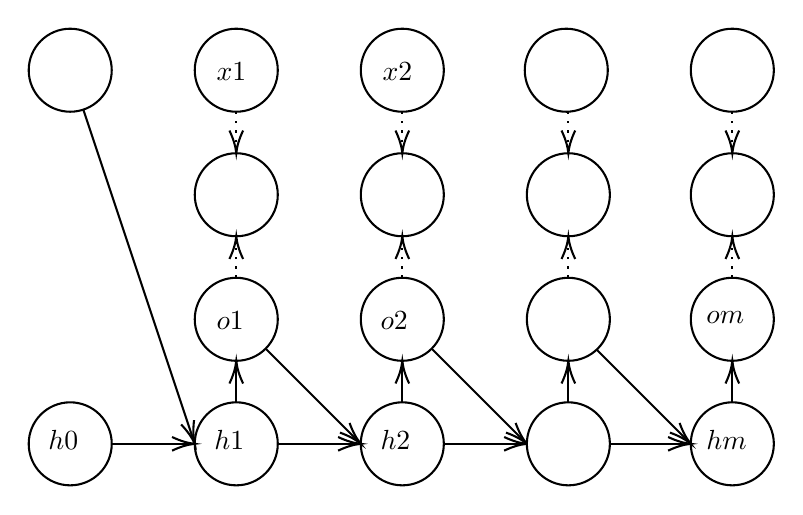
\begin{tikzpicture}[x=0.75pt,y=0.75pt,yscale=-1,xscale=1]
%uncomment if require: \path (0,300); %set diagram left start at 0, and has height of 300

%Straight Lines [id:da3705753956989253] 
\draw    (220,190) -- (278.59,248.59) ;
\draw [shift={(280,250)}, rotate = 225] [color={rgb, 255:red, 0; green, 0; blue, 0 }  ][line width=0.75]    (10.93,-3.29) .. controls (6.95,-1.4) and (3.31,-0.3) .. (0,0) .. controls (3.31,0.3) and (6.95,1.4) .. (10.93,3.29)   ;
%Straight Lines [id:da13768476860068835] 
\draw    (140,190) -- (198.59,248.59) ;
\draw [shift={(200,250)}, rotate = 225] [color={rgb, 255:red, 0; green, 0; blue, 0 }  ][line width=0.75]    (10.93,-3.29) .. controls (6.95,-1.4) and (3.31,-0.3) .. (0,0) .. controls (3.31,0.3) and (6.95,1.4) .. (10.93,3.29)   ;
%Straight Lines [id:da7516734119726491] 
\draw    (60,70) -- (119.37,248.1) ;
\draw [shift={(120,250)}, rotate = 251.57] [color={rgb, 255:red, 0; green, 0; blue, 0 }  ][line width=0.75]    (10.93,-3.29) .. controls (6.95,-1.4) and (3.31,-0.3) .. (0,0) .. controls (3.31,0.3) and (6.95,1.4) .. (10.93,3.29)   ;
%Shape: Circle [id:dp2861374465427631] 
\draw  [fill={rgb, 255:red, 255; green, 255; blue, 255 }  ,fill opacity=1 ] (120,190) .. controls (120,178.95) and (128.95,170) .. (140,170) .. controls (151.05,170) and (160,178.95) .. (160,190) .. controls (160,201.05) and (151.05,210) .. (140,210) .. controls (128.95,210) and (120,201.05) .. (120,190) -- cycle ;
%Shape: Circle [id:dp8995746323333129] 
\draw  [fill={rgb, 255:red, 255; green, 255; blue, 255 }  ,fill opacity=1 ] (200,190) .. controls (200,178.95) and (208.95,170) .. (220,170) .. controls (231.05,170) and (240,178.95) .. (240,190) .. controls (240,201.05) and (231.05,210) .. (220,210) .. controls (208.95,210) and (200,201.05) .. (200,190) -- cycle ;
%Shape: Circle [id:dp5132847039135391] 
\draw   (359,190) .. controls (359,178.95) and (367.95,170) .. (379,170) .. controls (390.05,170) and (399,178.95) .. (399,190) .. controls (399,201.05) and (390.05,210) .. (379,210) .. controls (367.95,210) and (359,201.05) .. (359,190) -- cycle ;
%Shape: Circle [id:dp6883637705260288] 
\draw   (120,250) .. controls (120,238.95) and (128.95,230) .. (140,230) .. controls (151.05,230) and (160,238.95) .. (160,250) .. controls (160,261.05) and (151.05,270) .. (140,270) .. controls (128.95,270) and (120,261.05) .. (120,250) -- cycle ;
%Shape: Circle [id:dp012945078339698046] 
\draw   (200,250) .. controls (200,238.95) and (208.95,230) .. (220,230) .. controls (231.05,230) and (240,238.95) .. (240,250) .. controls (240,261.05) and (231.05,270) .. (220,270) .. controls (208.95,270) and (200,261.05) .. (200,250) -- cycle ;
%Shape: Circle [id:dp8758578688441847] 
\draw   (359,250) .. controls (359,238.95) and (367.95,230) .. (379,230) .. controls (390.05,230) and (399,238.95) .. (399,250) .. controls (399,261.05) and (390.05,270) .. (379,270) .. controls (367.95,270) and (359,261.05) .. (359,250) -- cycle ;
%Shape: Circle [id:dp9985863104435384] 
\draw   (120,130) .. controls (120,118.95) and (128.95,110) .. (140,110) .. controls (151.05,110) and (160,118.95) .. (160,130) .. controls (160,141.05) and (151.05,150) .. (140,150) .. controls (128.95,150) and (120,141.05) .. (120,130) -- cycle ;
%Shape: Circle [id:dp4455674204725262] 
\draw   (200,130) .. controls (200,118.95) and (208.95,110) .. (220,110) .. controls (231.05,110) and (240,118.95) .. (240,130) .. controls (240,141.05) and (231.05,150) .. (220,150) .. controls (208.95,150) and (200,141.05) .. (200,130) -- cycle ;
%Shape: Circle [id:dp29444715698499846] 
\draw   (359,130) .. controls (359,118.95) and (367.95,110) .. (379,110) .. controls (390.05,110) and (399,118.95) .. (399,130) .. controls (399,141.05) and (390.05,150) .. (379,150) .. controls (367.95,150) and (359,141.05) .. (359,130) -- cycle ;
%Shape: Circle [id:dp46907010739358745] 
\draw  [fill={rgb, 255:red, 255; green, 255; blue, 255 }  ,fill opacity=1 ] (40,70) .. controls (40,58.95) and (48.95,50) .. (60,50) .. controls (71.05,50) and (80,58.95) .. (80,70) .. controls (80,81.05) and (71.05,90) .. (60,90) .. controls (48.95,90) and (40,81.05) .. (40,70) -- cycle ;
%Shape: Circle [id:dp7881937002294943] 
\draw   (120,70) .. controls (120,58.95) and (128.95,50) .. (140,50) .. controls (151.05,50) and (160,58.95) .. (160,70) .. controls (160,81.05) and (151.05,90) .. (140,90) .. controls (128.95,90) and (120,81.05) .. (120,70) -- cycle ;
%Shape: Circle [id:dp7553352123696904] 
\draw   (40,250) .. controls (40,238.95) and (48.95,230) .. (60,230) .. controls (71.05,230) and (80,238.95) .. (80,250) .. controls (80,261.05) and (71.05,270) .. (60,270) .. controls (48.95,270) and (40,261.05) .. (40,250) -- cycle ;
%Shape: Circle [id:dp010471915003695598] 
\draw   (359,70) .. controls (359,58.95) and (367.95,50) .. (379,50) .. controls (390.05,50) and (399,58.95) .. (399,70) .. controls (399,81.05) and (390.05,90) .. (379,90) .. controls (367.95,90) and (359,81.05) .. (359,70) -- cycle ;
%Straight Lines [id:da7216075417917613] 
\draw    (80,250) -- (118,250) ;
\draw [shift={(120,250)}, rotate = 180] [color={rgb, 255:red, 0; green, 0; blue, 0 }  ][line width=0.75]    (10.93,-3.29) .. controls (6.95,-1.4) and (3.31,-0.3) .. (0,0) .. controls (3.31,0.3) and (6.95,1.4) .. (10.93,3.29)   ;
%Straight Lines [id:da07185232587621804] 
\draw    (160,250) -- (198,250) ;
\draw [shift={(200,250)}, rotate = 180] [color={rgb, 255:red, 0; green, 0; blue, 0 }  ][line width=0.75]    (10.93,-3.29) .. controls (6.95,-1.4) and (3.31,-0.3) .. (0,0) .. controls (3.31,0.3) and (6.95,1.4) .. (10.93,3.29)   ;
%Straight Lines [id:da7244113775322998] 
\draw    (319,250) -- (357,250) ;
\draw [shift={(359,250)}, rotate = 180] [color={rgb, 255:red, 0; green, 0; blue, 0 }  ][line width=0.75]    (10.93,-3.29) .. controls (6.95,-1.4) and (3.31,-0.3) .. (0,0) .. controls (3.31,0.3) and (6.95,1.4) .. (10.93,3.29)   ;
%Straight Lines [id:da24576051067119886] 
\draw    (140,230) -- (140,212) ;
\draw [shift={(140,210)}, rotate = 450] [color={rgb, 255:red, 0; green, 0; blue, 0 }  ][line width=0.75]    (10.93,-3.29) .. controls (6.95,-1.4) and (3.31,-0.3) .. (0,0) .. controls (3.31,0.3) and (6.95,1.4) .. (10.93,3.29)   ;
%Straight Lines [id:da7265276007326142] 
\draw    (220,230) -- (220,212) ;
\draw [shift={(220,210)}, rotate = 450] [color={rgb, 255:red, 0; green, 0; blue, 0 }  ][line width=0.75]    (10.93,-3.29) .. controls (6.95,-1.4) and (3.31,-0.3) .. (0,0) .. controls (3.31,0.3) and (6.95,1.4) .. (10.93,3.29)   ;
%Straight Lines [id:da2431010870132262] 
\draw    (379,230) -- (379,212) ;
\draw [shift={(379,210)}, rotate = 450] [color={rgb, 255:red, 0; green, 0; blue, 0 }  ][line width=0.75]    (10.93,-3.29) .. controls (6.95,-1.4) and (3.31,-0.3) .. (0,0) .. controls (3.31,0.3) and (6.95,1.4) .. (10.93,3.29)   ;
%Straight Lines [id:da8493376218977626] 
\draw  [dash pattern={on 0.84pt off 2.51pt}]  (140,170) -- (140,152) ;
\draw [shift={(140,150)}, rotate = 450] [color={rgb, 255:red, 0; green, 0; blue, 0 }  ][line width=0.75]    (10.93,-3.29) .. controls (6.95,-1.4) and (3.31,-0.3) .. (0,0) .. controls (3.31,0.3) and (6.95,1.4) .. (10.93,3.29)   ;
%Straight Lines [id:da3483328514153865] 
\draw  [dash pattern={on 0.84pt off 2.51pt}]  (220,170) -- (220,152) ;
\draw [shift={(220,150)}, rotate = 450] [color={rgb, 255:red, 0; green, 0; blue, 0 }  ][line width=0.75]    (10.93,-3.29) .. controls (6.95,-1.4) and (3.31,-0.3) .. (0,0) .. controls (3.31,0.3) and (6.95,1.4) .. (10.93,3.29)   ;
%Straight Lines [id:da41996776114892587] 
\draw  [dash pattern={on 0.84pt off 2.51pt}]  (379,170) -- (379,152) ;
\draw [shift={(379,150)}, rotate = 450] [color={rgb, 255:red, 0; green, 0; blue, 0 }  ][line width=0.75]    (10.93,-3.29) .. controls (6.95,-1.4) and (3.31,-0.3) .. (0,0) .. controls (3.31,0.3) and (6.95,1.4) .. (10.93,3.29)   ;
%Straight Lines [id:da6136891468012544] 
\draw  [dash pattern={on 0.84pt off 2.51pt}]  (140,90) -- (140,108) ;
\draw [shift={(140,110)}, rotate = 270] [color={rgb, 255:red, 0; green, 0; blue, 0 }  ][line width=0.75]    (10.93,-3.29) .. controls (6.95,-1.4) and (3.31,-0.3) .. (0,0) .. controls (3.31,0.3) and (6.95,1.4) .. (10.93,3.29)   ;
%Straight Lines [id:da5904233910773451] 
\draw  [dash pattern={on 0.84pt off 2.51pt}]  (220,90) -- (220,108) ;
\draw [shift={(220,110)}, rotate = 270] [color={rgb, 255:red, 0; green, 0; blue, 0 }  ][line width=0.75]    (10.93,-3.29) .. controls (6.95,-1.4) and (3.31,-0.3) .. (0,0) .. controls (3.31,0.3) and (6.95,1.4) .. (10.93,3.29)   ;
%Straight Lines [id:da5897157922315699] 
\draw  [dash pattern={on 0.84pt off 2.51pt}]  (379,90) -- (379,108) ;
\draw [shift={(379,110)}, rotate = 270] [color={rgb, 255:red, 0; green, 0; blue, 0 }  ][line width=0.75]    (10.93,-3.29) .. controls (6.95,-1.4) and (3.31,-0.3) .. (0,0) .. controls (3.31,0.3) and (6.95,1.4) .. (10.93,3.29)   ;
%Straight Lines [id:da8515776227334051] 
\draw    (240,250) -- (278,250) ;
\draw [shift={(280,250)}, rotate = 180] [color={rgb, 255:red, 0; green, 0; blue, 0 }  ][line width=0.75]    (10.93,-3.29) .. controls (6.95,-1.4) and (3.31,-0.3) .. (0,0) .. controls (3.31,0.3) and (6.95,1.4) .. (10.93,3.29)   ;
%Straight Lines [id:da6960605501599442] 
\draw    (299,190) -- (357.59,248.59) ;
\draw [shift={(359,250)}, rotate = 225] [color={rgb, 255:red, 0; green, 0; blue, 0 }  ][line width=0.75]    (10.93,-3.29) .. controls (6.95,-1.4) and (3.31,-0.3) .. (0,0) .. controls (3.31,0.3) and (6.95,1.4) .. (10.93,3.29)   ;
%Shape: Circle [id:dp6682696219164692] 
\draw   (200,70) .. controls (200,58.95) and (208.95,50) .. (220,50) .. controls (231.05,50) and (240,58.95) .. (240,70) .. controls (240,81.05) and (231.05,90) .. (220,90) .. controls (208.95,90) and (200,81.05) .. (200,70) -- cycle ;
%Shape: Circle [id:dp504248140391159] 
\draw  [color={rgb, 255:red, 0; green, 0; blue, 0 }  ,draw opacity=1 ][fill={rgb, 255:red, 255; green, 255; blue, 255 }  ,fill opacity=1 ] (280,250) .. controls (280,238.95) and (288.95,230) .. (300,230) .. controls (311.05,230) and (320,238.95) .. (320,250) .. controls (320,261.05) and (311.05,270) .. (300,270) .. controls (288.95,270) and (280,261.05) .. (280,250) -- cycle ;
%Shape: Circle [id:dp6268313110219861] 
\draw  [color={rgb, 255:red, 0; green, 0; blue, 0 }  ,draw opacity=1 ][fill={rgb, 255:red, 255; green, 255; blue, 255 }  ,fill opacity=1 ] (280,190) .. controls (280,178.95) and (288.95,170) .. (300,170) .. controls (311.05,170) and (320,178.95) .. (320,190) .. controls (320,201.05) and (311.05,210) .. (300,210) .. controls (288.95,210) and (280,201.05) .. (280,190) -- cycle ;
%Shape: Circle [id:dp18481290998458055] 
\draw  [color={rgb, 255:red, 0; green, 0; blue, 0 }  ,draw opacity=1 ][fill={rgb, 255:red, 255; green, 255; blue, 255 }  ,fill opacity=1 ] (280,130) .. controls (280,118.95) and (288.95,110) .. (300,110) .. controls (311.05,110) and (320,118.95) .. (320,130) .. controls (320,141.05) and (311.05,150) .. (300,150) .. controls (288.95,150) and (280,141.05) .. (280,130) -- cycle ;
%Shape: Circle [id:dp38894485526229583] 
\draw  [color={rgb, 255:red, 0; green, 0; blue, 0 }  ,draw opacity=1 ][fill={rgb, 255:red, 255; green, 255; blue, 255 }  ,fill opacity=1 ] (279,70) .. controls (279,58.95) and (287.95,50) .. (299,50) .. controls (310.05,50) and (319,58.95) .. (319,70) .. controls (319,81.05) and (310.05,90) .. (299,90) .. controls (287.95,90) and (279,81.05) .. (279,70) -- cycle ;
%Straight Lines [id:da37604334047185195] 
\draw    (300,230) -- (300,212) ;
\draw [shift={(300,210)}, rotate = 450] [color={rgb, 255:red, 0; green, 0; blue, 0 }  ][line width=0.75]    (10.93,-3.29) .. controls (6.95,-1.4) and (3.31,-0.3) .. (0,0) .. controls (3.31,0.3) and (6.95,1.4) .. (10.93,3.29)   ;
%Straight Lines [id:da5744451958950472] 
\draw  [dash pattern={on 0.84pt off 2.51pt}]  (300,170) -- (300,152) ;
\draw [shift={(300,150)}, rotate = 450] [color={rgb, 255:red, 0; green, 0; blue, 0 }  ][line width=0.75]    (10.93,-3.29) .. controls (6.95,-1.4) and (3.31,-0.3) .. (0,0) .. controls (3.31,0.3) and (6.95,1.4) .. (10.93,3.29)   ;
%Straight Lines [id:da5213392331437636] 
\draw  [dash pattern={on 0.84pt off 2.51pt}]  (300,90) -- (300,108) ;
\draw [shift={(300,110)}, rotate = 270] [color={rgb, 255:red, 0; green, 0; blue, 0 }  ][line width=0.75]    (10.93,-3.29) .. controls (6.95,-1.4) and (3.31,-0.3) .. (0,0) .. controls (3.31,0.3) and (6.95,1.4) .. (10.93,3.29)   ;

% Text Node
\draw (48,242) node [anchor=north west][inner sep=0.75pt]    {$\Elem{h}{0}$};
% Text Node
\draw (128,242) node [anchor=north west][inner sep=0.75pt]    {$\Elem{h}{1}$};
% Text Node
\draw (208,242) node [anchor=north west][inner sep=0.75pt]    {$\Elem{h}{2}$};
% Text Node
\draw (290,247) node [anchor=north west][inner sep=0.75pt]    {$\dotsc $};
% Text Node
\draw (365,242) node [anchor=north west][inner sep=0.75pt]    {$\Elem{h}{m}$};

% Text Node
\draw (129,185) node [anchor=north west][inner sep=0.75pt]    {$\Elem{o}{1}$};
% Text Node
\draw (208,185) node [anchor=north west][inner sep=0.75pt]    {$\Elem{o}{2}$};
% Text Node
\draw (290,188) node [anchor=north west][inner sep=0.75pt]    {$\dotsc $};
% Text Node
\draw (365,185) node [anchor=north west][inner sep=0.75pt]    {$\Elem{o}{m}$};

% Text Node
\draw (133,123) node [anchor=north west][inner sep=0.75pt]    {$\Loss$};
% Text Node
\draw (213,123) node [anchor=north west][inner sep=0.75pt]    {$\Loss$};
% Text Node
\draw (293,123) node [anchor=north west][inner sep=0.75pt]    {$\Loss$};
% Text Node
\draw (372,123) node [anchor=north west][inner sep=0.75pt]    {$\Loss$};

% Text Node
\draw (43,62.5) node [anchor=north west][inner sep=0.75pt]  [font=\small]  {$\SOS$};
% Text Node
\draw (129,65) node [anchor=north west][inner sep=0.75pt]    {$\Elem{x}{1}$};
% Text Node
\draw (209,65) node [anchor=north west][inner sep=0.75pt]    {$\Elem{x}{2}$};
% Text Node
\draw (290,68) node [anchor=north west][inner sep=0.75pt]    {$\dotsc $};
% Text Node
\draw (362,62.5) node [anchor=north west][inner sep=0.75pt]  [font=\small]  {$\EOS$};

\end{tikzpicture}}
        \caption{}
        \label{fig:auto-regressive}
    \end{subfigure}
    \begin{subfigure}[b]{0.49\linewidth}
        \centering
        \resizebox{.9\textwidth}{!}{

\tikzset{every picture/.style={line width=0.75pt}} %set default line width to 0.75pt

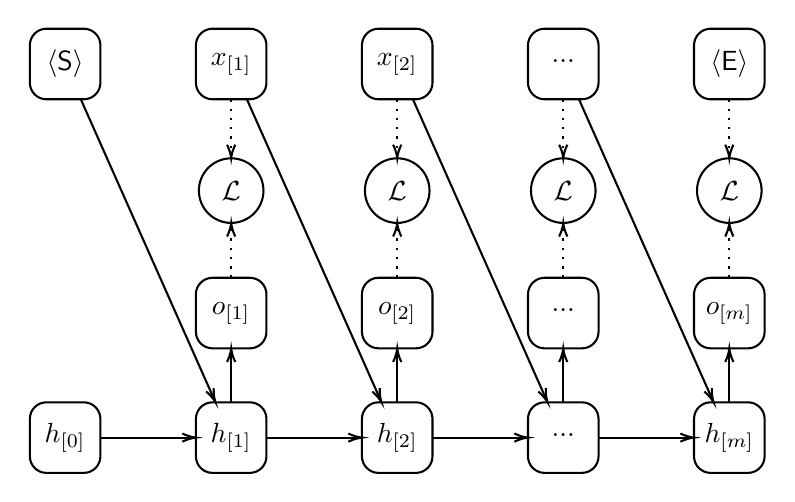
\begin{tikzpicture}[x=0.75pt,y=0.75pt,yscale=-1,xscale=1]
%uncomment if require: \path (0,259); %set diagram left start at 0, and has height of 259


% Text Node
\draw  [fill={rgb, 255:red, 255; green, 255; blue, 255 }  ,fill opacity=1 ]  (138,221) .. controls (138,216.58) and (141.58,213) .. (146,213) -- (164,213) .. controls (168.42,213) and (172,216.58) .. (172,221) -- (172,239) .. controls (172,243.42) and (168.42,247) .. (164,247) -- (146,247) .. controls (141.58,247) and (138,243.42) .. (138,239) -- cycle  ;
\draw (155,230) node   [align=left] {\begin{minipage}[lt]{20.400000000000002pt}\setlength\topsep{0pt}
\begin{center}
$\displaystyle \boldsymbol{h}_{[ 1]}$
\end{center}

\end{minipage}};
% Text Node
\draw    (58,221) .. controls (58,216.58) and (61.58,213) .. (66,213) -- (84,213) .. controls (88.42,213) and (92,216.58) .. (92,221) -- (92,239) .. controls (92,243.42) and (88.42,247) .. (84,247) -- (66,247) .. controls (61.58,247) and (58,243.42) .. (58,239) -- cycle  ;
\draw (75,230) node   [align=left] {\begin{minipage}[lt]{20.400000000000002pt}\setlength\topsep{0pt}
\begin{center}
$\displaystyle \boldsymbol{h}_{[ 0]}$
\end{center}

\end{minipage}};
% Text Node
\draw    (138,161) .. controls (138,156.58) and (141.58,153) .. (146,153) -- (164,153) .. controls (168.42,153) and (172,156.58) .. (172,161) -- (172,179) .. controls (172,183.42) and (168.42,187) .. (164,187) -- (146,187) .. controls (141.58,187) and (138,183.42) .. (138,179) -- cycle  ;
\draw (155,170) node   [align=left] {\begin{minipage}[lt]{20.400000000000002pt}\setlength\topsep{0pt}
\begin{center}
$\displaystyle \boldsymbol{o}_{[ 1]}$
\end{center}

\end{minipage}};
% Text Node
\draw    (138,41) .. controls (138,36.58) and (141.58,33) .. (146,33) -- (164,33) .. controls (168.42,33) and (172,36.58) .. (172,41) -- (172,59) .. controls (172,63.42) and (168.42,67) .. (164,67) -- (146,67) .. controls (141.58,67) and (138,63.42) .. (138,59) -- cycle  ;
\draw (155,50) node   [align=left] {\begin{minipage}[lt]{20.400000000000002pt}\setlength\topsep{0pt}
\begin{center}
$\displaystyle \boldsymbol{x}_{[ 1]}$
\end{center}

\end{minipage}};
% Text Node
\draw  [fill={rgb, 255:red, 255; green, 255; blue, 255 }  ,fill opacity=1 ]  (218,221) .. controls (218,216.58) and (221.58,213) .. (226,213) -- (244,213) .. controls (248.42,213) and (252,216.58) .. (252,221) -- (252,239) .. controls (252,243.42) and (248.42,247) .. (244,247) -- (226,247) .. controls (221.58,247) and (218,243.42) .. (218,239) -- cycle  ;
\draw (235,230) node   [align=left] {\begin{minipage}[lt]{20.400000000000002pt}\setlength\topsep{0pt}
\begin{center}
$\displaystyle \boldsymbol{h}_{[ 2]}$
\end{center}

\end{minipage}};
% Text Node
\draw    (218,161) .. controls (218,156.58) and (221.58,153) .. (226,153) -- (244,153) .. controls (248.42,153) and (252,156.58) .. (252,161) -- (252,179) .. controls (252,183.42) and (248.42,187) .. (244,187) -- (226,187) .. controls (221.58,187) and (218,183.42) .. (218,179) -- cycle  ;
\draw (235,170) node   [align=left] {\begin{minipage}[lt]{20.400000000000002pt}\setlength\topsep{0pt}
\begin{center}
$\displaystyle \boldsymbol{o}_{[ 2]}$
\end{center}

\end{minipage}};
% Text Node
\draw    (218,41) .. controls (218,36.58) and (221.58,33) .. (226,33) -- (244,33) .. controls (248.42,33) and (252,36.58) .. (252,41) -- (252,59) .. controls (252,63.42) and (248.42,67) .. (244,67) -- (226,67) .. controls (221.58,67) and (218,63.42) .. (218,59) -- cycle  ;
\draw (235,50) node   [align=left] {\begin{minipage}[lt]{20.400000000000002pt}\setlength\topsep{0pt}
\begin{center}
$\displaystyle \boldsymbol{x}_{[ 2]}$
\end{center}

\end{minipage}};
% Text Node
\draw  [fill={rgb, 255:red, 255; green, 255; blue, 255 }  ,fill opacity=1 ]  (298,221) .. controls (298,216.58) and (301.58,213) .. (306,213) -- (324,213) .. controls (328.42,213) and (332,216.58) .. (332,221) -- (332,239) .. controls (332,243.42) and (328.42,247) .. (324,247) -- (306,247) .. controls (301.58,247) and (298,243.42) .. (298,239) -- cycle  ;
\draw (315,230) node   [align=left] {\begin{minipage}[lt]{20.400000000000002pt}\setlength\topsep{0pt}
\begin{center}
$\displaystyle ...$
\end{center}

\end{minipage}};
% Text Node
\draw    (298,161) .. controls (298,156.58) and (301.58,153) .. (306,153) -- (324,153) .. controls (328.42,153) and (332,156.58) .. (332,161) -- (332,179) .. controls (332,183.42) and (328.42,187) .. (324,187) -- (306,187) .. controls (301.58,187) and (298,183.42) .. (298,179) -- cycle  ;
\draw (315,170) node   [align=left] {\begin{minipage}[lt]{20.400000000000002pt}\setlength\topsep{0pt}
\begin{center}
$\displaystyle ...$
\end{center}

\end{minipage}};
% Text Node
\draw    (298,41) .. controls (298,36.58) and (301.58,33) .. (306,33) -- (324,33) .. controls (328.42,33) and (332,36.58) .. (332,41) -- (332,59) .. controls (332,63.42) and (328.42,67) .. (324,67) -- (306,67) .. controls (301.58,67) and (298,63.42) .. (298,59) -- cycle  ;
\draw (315,50) node   [align=left] {\begin{minipage}[lt]{20.400000000000002pt}\setlength\topsep{0pt}
\begin{center}
$\displaystyle ...$
\end{center}

\end{minipage}};
% Text Node
\draw  [fill={rgb, 255:red, 255; green, 255; blue, 255 }  ,fill opacity=1 ]  (378,221) .. controls (378,216.58) and (381.58,213) .. (386,213) -- (404,213) .. controls (408.42,213) and (412,216.58) .. (412,221) -- (412,239) .. controls (412,243.42) and (408.42,247) .. (404,247) -- (386,247) .. controls (381.58,247) and (378,243.42) .. (378,239) -- cycle  ;
\draw (395,230) node   [align=left] {\begin{minipage}[lt]{20.400000000000002pt}\setlength\topsep{0pt}
\begin{center}
$\displaystyle \boldsymbol{h}_{[ m]}$
\end{center}

\end{minipage}};
% Text Node
\draw    (378,161) .. controls (378,156.58) and (381.58,153) .. (386,153) -- (404,153) .. controls (408.42,153) and (412,156.58) .. (412,161) -- (412,179) .. controls (412,183.42) and (408.42,187) .. (404,187) -- (386,187) .. controls (381.58,187) and (378,183.42) .. (378,179) -- cycle  ;
\draw (395,170) node   [align=left] {\begin{minipage}[lt]{20.400000000000002pt}\setlength\topsep{0pt}
\begin{center}
$\displaystyle \boldsymbol{o}_{[ m]}$
\end{center}

\end{minipage}};
% Text Node
\draw    (378,41) .. controls (378,36.58) and (381.58,33) .. (386,33) -- (404,33) .. controls (408.42,33) and (412,36.58) .. (412,41) -- (412,59) .. controls (412,63.42) and (408.42,67) .. (404,67) -- (386,67) .. controls (381.58,67) and (378,63.42) .. (378,59) -- cycle  ;
\draw (395,50) node   [align=left] {\begin{minipage}[lt]{20.400000000000002pt}\setlength\topsep{0pt}
\begin{center}
$\displaystyle \langle \mathsf{E} \rangle $
\end{center}

\end{minipage}};
% Text Node
\draw    (58,41) .. controls (58,36.58) and (61.58,33) .. (66,33) -- (84,33) .. controls (88.42,33) and (92,36.58) .. (92,41) -- (92,59) .. controls (92,63.42) and (88.42,67) .. (84,67) -- (66,67) .. controls (61.58,67) and (58,63.42) .. (58,59) -- cycle  ;
\draw (75,50) node   [align=left] {\begin{minipage}[lt]{20.400000000000002pt}\setlength\topsep{0pt}
\begin{center}
$\displaystyle \langle \mathsf{S} \rangle $
\end{center}

\end{minipage}};
% Text Node
\draw    (395, 111) circle [x radius= 15.56, y radius= 15.56]   ;
\draw (395,111) node   [align=left] {\begin{minipage}[lt]{13.735995849609345pt}\setlength\topsep{0pt}
\begin{center}
$\displaystyle \mathcal{L}$
\end{center}

\end{minipage}};
% Text Node
\draw    (315, 111) circle [x radius= 15.56, y radius= 15.56]   ;
\draw (315,111) node   [align=left] {\begin{minipage}[lt]{13.735995849609345pt}\setlength\topsep{0pt}
\begin{center}
$\displaystyle \mathcal{L}$
\end{center}

\end{minipage}};
% Text Node
\draw    (235, 111) circle [x radius= 15.56, y radius= 15.56]   ;
\draw (235,111) node   [align=left] {\begin{minipage}[lt]{13.735995849609345pt}\setlength\topsep{0pt}
\begin{center}
$\displaystyle \mathcal{L}$
\end{center}

\end{minipage}};
% Text Node
\draw    (155, 111) circle [x radius= 15.56, y radius= 15.56]   ;
\draw (155,111) node   [align=left] {\begin{minipage}[lt]{13.735995849609345pt}\setlength\topsep{0pt}
\begin{center}
$\displaystyle \mathcal{L}$
\end{center}

\end{minipage}};
% Connection
\draw    (92,230) -- (136,230) ;
\draw [shift={(138,230)}, rotate = 180] [color={rgb, 255:red, 0; green, 0; blue, 0 }  ][line width=0.75]    (6.56,-1.97) .. controls (4.17,-0.84) and (1.99,-0.18) .. (0,0) .. controls (1.99,0.18) and (4.17,0.84) .. (6.56,1.97)   ;
% Connection
\draw    (155,213) -- (155,189) ;
\draw [shift={(155,187)}, rotate = 450] [color={rgb, 255:red, 0; green, 0; blue, 0 }  ][line width=0.75]    (6.56,-1.97) .. controls (4.17,-0.84) and (1.99,-0.18) .. (0,0) .. controls (1.99,0.18) and (4.17,0.84) .. (6.56,1.97)   ;
% Connection
\draw    (235,213) -- (235,189) ;
\draw [shift={(235,187)}, rotate = 450] [color={rgb, 255:red, 0; green, 0; blue, 0 }  ][line width=0.75]    (6.56,-1.97) .. controls (4.17,-0.84) and (1.99,-0.18) .. (0,0) .. controls (1.99,0.18) and (4.17,0.84) .. (6.56,1.97)   ;
% Connection
\draw    (172,230) -- (216,230) ;
\draw [shift={(218,230)}, rotate = 180] [color={rgb, 255:red, 0; green, 0; blue, 0 }  ][line width=0.75]    (6.56,-1.97) .. controls (4.17,-0.84) and (1.99,-0.18) .. (0,0) .. controls (1.99,0.18) and (4.17,0.84) .. (6.56,1.97)   ;
% Connection
\draw    (315,213) -- (315,189) ;
\draw [shift={(315,187)}, rotate = 450] [color={rgb, 255:red, 0; green, 0; blue, 0 }  ][line width=0.75]    (6.56,-1.97) .. controls (4.17,-0.84) and (1.99,-0.18) .. (0,0) .. controls (1.99,0.18) and (4.17,0.84) .. (6.56,1.97)   ;
% Connection
\draw    (252,230) -- (296,230) ;
\draw [shift={(298,230)}, rotate = 180] [color={rgb, 255:red, 0; green, 0; blue, 0 }  ][line width=0.75]    (6.56,-1.97) .. controls (4.17,-0.84) and (1.99,-0.18) .. (0,0) .. controls (1.99,0.18) and (4.17,0.84) .. (6.56,1.97)   ;
% Connection
\draw    (395,213) -- (395,189) ;
\draw [shift={(395,187)}, rotate = 450] [color={rgb, 255:red, 0; green, 0; blue, 0 }  ][line width=0.75]    (6.56,-1.97) .. controls (4.17,-0.84) and (1.99,-0.18) .. (0,0) .. controls (1.99,0.18) and (4.17,0.84) .. (6.56,1.97)   ;
% Connection
\draw    (332,230) -- (376,230) ;
\draw [shift={(378,230)}, rotate = 180] [color={rgb, 255:red, 0; green, 0; blue, 0 }  ][line width=0.75]    (6.56,-1.97) .. controls (4.17,-0.84) and (1.99,-0.18) .. (0,0) .. controls (1.99,0.18) and (4.17,0.84) .. (6.56,1.97)   ;
% Connection
\draw    (82.56,67) -- (146.63,211.17) ;
\draw [shift={(147.44,213)}, rotate = 246.04000000000002] [color={rgb, 255:red, 0; green, 0; blue, 0 }  ][line width=0.75]    (6.56,-1.97) .. controls (4.17,-0.84) and (1.99,-0.18) .. (0,0) .. controls (1.99,0.18) and (4.17,0.84) .. (6.56,1.97)   ;
% Connection
\draw    (162.56,67) -- (226.63,211.17) ;
\draw [shift={(227.44,213)}, rotate = 246.04000000000002] [color={rgb, 255:red, 0; green, 0; blue, 0 }  ][line width=0.75]    (6.56,-1.97) .. controls (4.17,-0.84) and (1.99,-0.18) .. (0,0) .. controls (1.99,0.18) and (4.17,0.84) .. (6.56,1.97)   ;
% Connection
\draw    (242.56,67) -- (306.63,211.17) ;
\draw [shift={(307.44,213)}, rotate = 246.04000000000002] [color={rgb, 255:red, 0; green, 0; blue, 0 }  ][line width=0.75]    (6.56,-1.97) .. controls (4.17,-0.84) and (1.99,-0.18) .. (0,0) .. controls (1.99,0.18) and (4.17,0.84) .. (6.56,1.97)   ;
% Connection
\draw    (322.56,67) -- (386.63,211.17) ;
\draw [shift={(387.44,213)}, rotate = 246.04000000000002] [color={rgb, 255:red, 0; green, 0; blue, 0 }  ][line width=0.75]    (6.56,-1.97) .. controls (4.17,-0.84) and (1.99,-0.18) .. (0,0) .. controls (1.99,0.18) and (4.17,0.84) .. (6.56,1.97)   ;
% Connection
\draw  [dash pattern={on 0.84pt off 2.51pt}]  (155,153) -- (155,128.56) ;
\draw [shift={(155,126.56)}, rotate = 450] [color={rgb, 255:red, 0; green, 0; blue, 0 }  ][line width=0.75]    (6.56,-1.97) .. controls (4.17,-0.84) and (1.99,-0.18) .. (0,0) .. controls (1.99,0.18) and (4.17,0.84) .. (6.56,1.97)   ;
% Connection
\draw  [dash pattern={on 0.84pt off 2.51pt}]  (155,67) -- (155,93.44) ;
\draw [shift={(155,95.44)}, rotate = 270] [color={rgb, 255:red, 0; green, 0; blue, 0 }  ][line width=0.75]    (6.56,-1.97) .. controls (4.17,-0.84) and (1.99,-0.18) .. (0,0) .. controls (1.99,0.18) and (4.17,0.84) .. (6.56,1.97)   ;
% Connection
\draw  [dash pattern={on 0.84pt off 2.51pt}]  (235,153) -- (235,128.56) ;
\draw [shift={(235,126.56)}, rotate = 450] [color={rgb, 255:red, 0; green, 0; blue, 0 }  ][line width=0.75]    (6.56,-1.97) .. controls (4.17,-0.84) and (1.99,-0.18) .. (0,0) .. controls (1.99,0.18) and (4.17,0.84) .. (6.56,1.97)   ;
% Connection
\draw  [dash pattern={on 0.84pt off 2.51pt}]  (235,67) -- (235,93.44) ;
\draw [shift={(235,95.44)}, rotate = 270] [color={rgb, 255:red, 0; green, 0; blue, 0 }  ][line width=0.75]    (6.56,-1.97) .. controls (4.17,-0.84) and (1.99,-0.18) .. (0,0) .. controls (1.99,0.18) and (4.17,0.84) .. (6.56,1.97)   ;
% Connection
\draw  [dash pattern={on 0.84pt off 2.51pt}]  (315,153) -- (315,128.56) ;
\draw [shift={(315,126.56)}, rotate = 450] [color={rgb, 255:red, 0; green, 0; blue, 0 }  ][line width=0.75]    (6.56,-1.97) .. controls (4.17,-0.84) and (1.99,-0.18) .. (0,0) .. controls (1.99,0.18) and (4.17,0.84) .. (6.56,1.97)   ;
% Connection
\draw  [dash pattern={on 0.84pt off 2.51pt}]  (315,67) -- (315,93.44) ;
\draw [shift={(315,95.44)}, rotate = 270] [color={rgb, 255:red, 0; green, 0; blue, 0 }  ][line width=0.75]    (6.56,-1.97) .. controls (4.17,-0.84) and (1.99,-0.18) .. (0,0) .. controls (1.99,0.18) and (4.17,0.84) .. (6.56,1.97)   ;
% Connection
\draw  [dash pattern={on 0.84pt off 2.51pt}]  (395,153) -- (395,128.56) ;
\draw [shift={(395,126.56)}, rotate = 450] [color={rgb, 255:red, 0; green, 0; blue, 0 }  ][line width=0.75]    (6.56,-1.97) .. controls (4.17,-0.84) and (1.99,-0.18) .. (0,0) .. controls (1.99,0.18) and (4.17,0.84) .. (6.56,1.97)   ;
% Connection
\draw  [dash pattern={on 0.84pt off 2.51pt}]  (395,67) -- (395,93.44) ;
\draw [shift={(395,95.44)}, rotate = 270] [color={rgb, 255:red, 0; green, 0; blue, 0 }  ][line width=0.75]    (6.56,-1.97) .. controls (4.17,-0.84) and (1.99,-0.18) .. (0,0) .. controls (1.99,0.18) and (4.17,0.84) .. (6.56,1.97)   ;

\end{tikzpicture}}
        \caption{}
        \label{fig:teacher-forcing}
    \end{subfigure}
    \caption{An example of training a recurrent neural network for learning an auto-regressive distribution. (A): standard training procedure. (B): training with teacher forcing.}
    \label{fig:rnn-auto-regressive}
\end{figure*}
Once the network is trained, novel sequences can be generated according to the following scheme:
\begin{itemize}
    \item start the generation process feeding the initial hidden state $\Elem{h}{0}$ and a \emph{start of sequence} token $\SOS$ as input to the network;
    \item the output $\Elem{o}{1}$ of the network is a distribution over sequence elements. Sample a new sequence element $\Elem{\tilde{x}}{1} \sim \Elem{o}{1}$;
    \item feed the updated hidden state $\Elem{h}{1}$ and the sampled element $\Elem{\tilde{x}}{1}$ as input to the network, and repeat the whole process until an \emph{end of sequence} token $\EOS$ is sampled;
    \item the generated sequence is $\tilde{S} = \Seq{\Elem{\tilde{x}}{1}, \Elem{\tilde{x}}{2}, \ldots}$.
\end{itemize}

\section{Recursive Neural Networks}
A \gls{recnn} is a \gls{nn} architecture that can adaptively process hierarchical data. Using trees as an example, let $T$ be a tree whose set of nodes is $\Cal{V}_T = \Set{v_1, v_2, \ldots, v_m}$, and let $T_{\Vector{x}} = \Set{\Elem{x}{v} \in \Real^d \mid v \in \Cal{V}_T}$ be its set node of features. The state transition function of a \gls{recnn}, applied locally to each node, is the following:
\begin{align*}
    \Elem{h}{v} &= \Transduction_{\Fun{enc}}(\Elem{x}{v}, \Elem{h}{S(v)}), \; \forall v \in \Cal{V}_T
\end{align*}
where $\Elem{h}{S(v)} \in \Real^h$ is the hidden state of the sub-tree rooted at $v$. As with \glspl{rnn}, the state transition function $\Transduction_{\Fun{enc}}$ is recursive, but this time the recursion is defined over the tree structure. Specifically, to compute the hidden state of a node, the hidden state of all its children must be known in advance. The state computation starts at the leaves of the tree (where the state is initialized beforehand to make the recursion well-defined), and proceeds bottom-up until the root node is reached.
The development of \glspl{recnn} started in the middle '90s \cite{?}, with the introduction of the notion of generalized recursive neuron \cite{?} and the development of a general framework for learning with tree-structured data \cite{?}, which was later extended to more expressive classes of structures such as \glspl{dag} and \glspl{dpag}. Since then, they have applied fruitfully in several fields, including among others cheminformatics \cite{?}, sentiment analysis \cite{?} and scene parsing \cite{?}. Interestingly, \glspl{recnn} are also backed up by strong theoretical results, which support the generality of the structural transduction and characterize the kind of functions they can learn. Specifically, universal approximation theorems showing that \glspl{recnn} can approximate arbitrarily well any function from labeled trees to real values \cite{?}, and from labelled \glspl{dpag} to real values \cite{?} have been proved.

\subsection{Training}
Using the binary tree of Figure \ref{fig:tree} and a structure-to-element task as an example, one possible implementation of the state transition function of a \gls{recnn} is the following:
\begin{align*}
    \Elem{h}{v} &= g\Paren{\Matrix{W}^{\Transpose}\Elem{x}{v} + \Matrix{U}_\Fun{l}^{\Transpose}\Elem{h}{\Fun{l}(v)} + \Matrix{U}_\Fun{r}^{\Transpose}\Elem{h}{\Fun{r}(v)}},\; \forall v \in \Cal{v}_{T}.
\end{align*} 
In the above formula, $g$ can be any hidden activation function, and $\Matrix{w} \in \Real^{d \times h}$, $\Matrix{u}_\Fun{l}$, and $\Matrix{u}_\Fun{r} \in \Real^{h \times h}$, are weight matrices shared across the structure. Notice that the two weight matrices on the node children are positional, meaning that they are applied to a certain node according to its position. In the example case of a binary tree, the two functions $\Fun{l}(v)$ and $\Fun{r}(v)$ select the left and right child of a node $v$, respectively, if they exist. Figure \ref{fig:recnn} shows the unfolded \gls{recnn} over the tree, where the final output of the entire structure is obtained using the hidden state of the root node $v_1$ as:
$$\Vector{o} = g_{\mathrm{out}}\Paren{\Elem{h}{v_1}},$$
where $\Vector{o} \in \Real^y$ is the output of the network and $g_{\mathrm{out}}$ can be any downstream network such as a simple output layer, or a more complex neural network. For structure-to-structure tasks, the output is calculated node-wise as follows:
$$\Elem{o}{v} = g_{\mathrm{out}}\Paren{\Elem{h}{v}},\; \forall v \in \Cal{v}_{T}.$$
Notably, the order by which the hidden states need to be calculated (the numbers at the left of the hidden states in the figure) must be respected to ensure that the recursive process is well-defined. The states of nodes with the same ordering can be calculated in parallel according to the tree structure, which makes \glspl{recnn} more efficient than \glspl{rnn} when compared on structures with the same number of elements.
\begin{figure*}[h!]
    \centering
    \resizebox{.5\textwidth}{!}{

\tikzset{every picture/.style={line width=0.75pt}} %set default line width to 0.75pt        

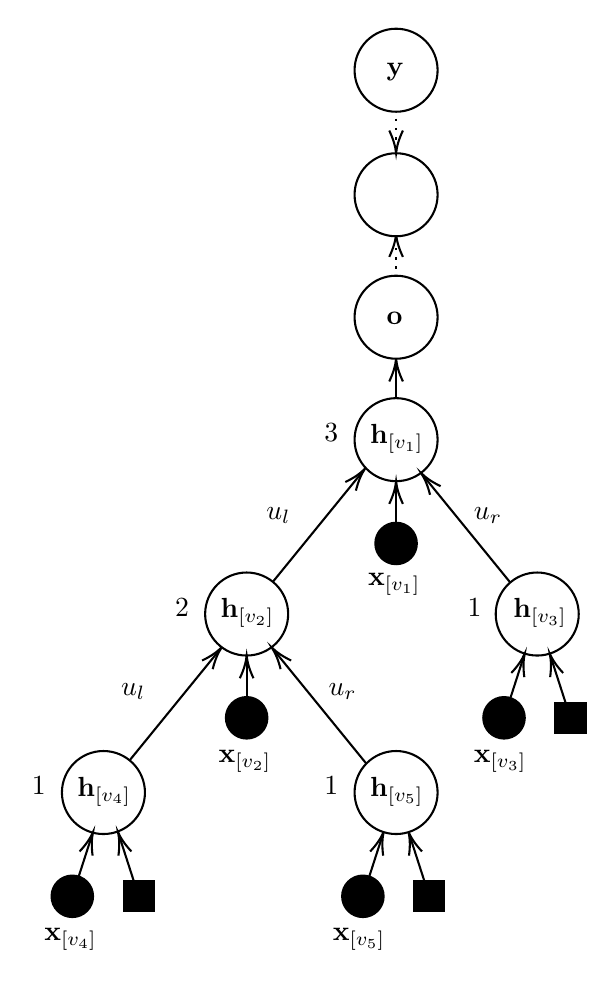
\begin{tikzpicture}[x=0.75pt,y=0.75pt,yscale=-1,xscale=1]
%uncomment if require: \path (0,492); %set diagram left start at 0, and has height of 492

%Straight Lines [id:da7466257393669937] 
\draw  [dash pattern={on 0.84pt off 2.51pt}]  (274,154) -- (274,117) ;
\draw [shift={(274,115)}, rotate = 450] [color={rgb, 255:red, 0; green, 0; blue, 0 }  ][line width=0.75]    (10.93,-3.29) .. controls (6.95,-1.4) and (3.31,-0.3) .. (0,0) .. controls (3.31,0.3) and (6.95,1.4) .. (10.93,3.29)   ;
%Straight Lines [id:da0893429759940223] 
\draw    (202,298) -- (257.74,229.55) ;
\draw [shift={(259,228)}, rotate = 489.16] [color={rgb, 255:red, 0; green, 0; blue, 0 }  ][line width=0.75]    (10.93,-3.29) .. controls (6.95,-1.4) and (3.31,-0.3) .. (0,0) .. controls (3.31,0.3) and (6.95,1.4) .. (10.93,3.29)   ;
%Straight Lines [id:da45368582829246695] 
\draw    (274,214) -- (274,177) ;
\draw [shift={(274,175)}, rotate = 450] [color={rgb, 255:red, 0; green, 0; blue, 0 }  ][line width=0.75]    (10.93,-3.29) .. controls (6.95,-1.4) and (3.31,-0.3) .. (0,0) .. controls (3.31,0.3) and (6.95,1.4) .. (10.93,3.29)   ;
%Straight Lines [id:da5078932225026183] 
\draw    (133,384) -- (188.74,315.55) ;
\draw [shift={(190,314)}, rotate = 489.16] [color={rgb, 255:red, 0; green, 0; blue, 0 }  ][line width=0.75]    (10.93,-3.29) .. controls (6.95,-1.4) and (3.31,-0.3) .. (0,0) .. controls (3.31,0.3) and (6.95,1.4) .. (10.93,3.29)   ;
%Shape: Circle [id:dp24012160731282295] 
\draw  [fill={rgb, 255:red, 255; green, 255; blue, 255 }  ,fill opacity=1 ] (182,298) .. controls (182,286.95) and (190.95,278) .. (202,278) .. controls (213.05,278) and (222,286.95) .. (222,298) .. controls (222,309.05) and (213.05,318) .. (202,318) .. controls (190.95,318) and (182,309.05) .. (182,298) -- cycle ;
%Shape: Circle [id:dp1550364357379772] 
\draw  [fill={rgb, 255:red, 0; green, 0; blue, 0 }  ,fill opacity=1 ] (192,348) .. controls (192,342.48) and (196.48,338) .. (202,338) .. controls (207.52,338) and (212,342.48) .. (212,348) .. controls (212,353.52) and (207.52,358) .. (202,358) .. controls (196.48,358) and (192,353.52) .. (192,348) -- cycle ;
%Shape: Boxed Line [id:dp6025172331519966] 
\draw    (202,358) -- (202,320) ;
\draw [shift={(202,318)}, rotate = 450] [color={rgb, 255:red, 0; green, 0; blue, 0 }  ][line width=0.75]    (10.93,-3.29) .. controls (6.95,-1.4) and (3.31,-0.3) .. (0,0) .. controls (3.31,0.3) and (6.95,1.4) .. (10.93,3.29)   ;
%Straight Lines [id:da8407999459301969] 
\draw    (271,384) -- (215.26,315.55) ;
\draw [shift={(214,314)}, rotate = 410.84000000000003] [color={rgb, 255:red, 0; green, 0; blue, 0 }  ][line width=0.75]    (10.93,-3.29) .. controls (6.95,-1.4) and (3.31,-0.3) .. (0,0) .. controls (3.31,0.3) and (6.95,1.4) .. (10.93,3.29)   ;
%Shape: Circle [id:dp07913655238390982] 
\draw  [fill={rgb, 255:red, 0; green, 0; blue, 0 }  ,fill opacity=1 ] (248,434) .. controls (248,428.48) and (252.48,424) .. (258,424) .. controls (263.52,424) and (268,428.48) .. (268,434) .. controls (268,439.52) and (263.52,444) .. (258,444) .. controls (252.48,444) and (248,439.52) .. (248,434) -- cycle ;
%Shape: Boxed Line [id:dp48364561900002645] 
\draw    (258,434) -- (267.39,404.9) ;
\draw [shift={(268,403)}, rotate = 467.88] [color={rgb, 255:red, 0; green, 0; blue, 0 }  ][line width=0.75]    (10.93,-3.29) .. controls (6.95,-1.4) and (3.31,-0.3) .. (0,0) .. controls (3.31,0.3) and (6.95,1.4) .. (10.93,3.29)   ;
%Shape: Square [id:dp1295344079832137] 
\draw  [fill={rgb, 255:red, 0; green, 0; blue, 0 }  ,fill opacity=1 ] (282.75,426.75) -- (297.25,426.75) -- (297.25,441.25) -- (282.75,441.25) -- cycle ;
%Straight Lines [id:da9879737182355028] 
\draw    (290,434) -- (280.61,404.9) ;
\draw [shift={(280,403)}, rotate = 432.12] [color={rgb, 255:red, 0; green, 0; blue, 0 }  ][line width=0.75]    (10.93,-3.29) .. controls (6.95,-1.4) and (3.31,-0.3) .. (0,0) .. controls (3.31,0.3) and (6.95,1.4) .. (10.93,3.29)   ;
%Shape: Circle [id:dp5451047636709254] 
\draw  [fill={rgb, 255:red, 255; green, 255; blue, 255 }  ,fill opacity=1 ] (153,384) .. controls (153,372.95) and (144.05,364) .. (133,364) .. controls (121.95,364) and (113,372.95) .. (113,384) .. controls (113,395.05) and (121.95,404) .. (133,404) .. controls (144.05,404) and (153,395.05) .. (153,384) -- cycle ;
%Shape: Circle [id:dp9493600152247126] 
\draw  [fill={rgb, 255:red, 255; green, 255; blue, 255 }  ,fill opacity=1 ] (254,214) .. controls (254,202.95) and (262.95,194) .. (274,194) .. controls (285.05,194) and (294,202.95) .. (294,214) .. controls (294,225.05) and (285.05,234) .. (274,234) .. controls (262.95,234) and (254,225.05) .. (254,214) -- cycle ;
%Shape: Circle [id:dp4891423949064355] 
\draw  [fill={rgb, 255:red, 0; green, 0; blue, 0 }  ,fill opacity=1 ] (264,264) .. controls (264,258.48) and (268.48,254) .. (274,254) .. controls (279.52,254) and (284,258.48) .. (284,264) .. controls (284,269.52) and (279.52,274) .. (274,274) .. controls (268.48,274) and (264,269.52) .. (264,264) -- cycle ;
%Shape: Boxed Line [id:dp5456540610731977] 
\draw    (274,274) -- (274,236) ;
\draw [shift={(274,234)}, rotate = 450] [color={rgb, 255:red, 0; green, 0; blue, 0 }  ][line width=0.75]    (10.93,-3.29) .. controls (6.95,-1.4) and (3.31,-0.3) .. (0,0) .. controls (3.31,0.3) and (6.95,1.4) .. (10.93,3.29)   ;
%Straight Lines [id:da23176333949094907] 
\draw    (343,300) -- (287.26,231.55) ;
\draw [shift={(286,230)}, rotate = 410.84000000000003] [color={rgb, 255:red, 0; green, 0; blue, 0 }  ][line width=0.75]    (10.93,-3.29) .. controls (6.95,-1.4) and (3.31,-0.3) .. (0,0) .. controls (3.31,0.3) and (6.95,1.4) .. (10.93,3.29)   ;
%Shape: Circle [id:dp8584128832152986] 
\draw  [fill={rgb, 255:red, 255; green, 255; blue, 255 }  ,fill opacity=1 ] (254,155) .. controls (254,143.95) and (262.95,135) .. (274,135) .. controls (285.05,135) and (294,143.95) .. (294,155) .. controls (294,166.05) and (285.05,175) .. (274,175) .. controls (262.95,175) and (254,166.05) .. (254,155) -- cycle ;
%Shape: Circle [id:dp2837295917607394] 
\draw  [fill={rgb, 255:red, 255; green, 255; blue, 255 }  ,fill opacity=1 ] (254,96) .. controls (254,84.95) and (262.95,76) .. (274,76) .. controls (285.05,76) and (294,84.95) .. (294,96) .. controls (294,107.05) and (285.05,116) .. (274,116) .. controls (262.95,116) and (254,107.05) .. (254,96) -- cycle ;
%Straight Lines [id:da45176985986405693] 
\draw  [dash pattern={on 0.84pt off 2.51pt}]  (274,37) -- (274,74) ;
\draw [shift={(274,76)}, rotate = 270] [color={rgb, 255:red, 0; green, 0; blue, 0 }  ][line width=0.75]    (10.93,-3.29) .. controls (6.95,-1.4) and (3.31,-0.3) .. (0,0) .. controls (3.31,0.3) and (6.95,1.4) .. (10.93,3.29)   ;
%Shape: Circle [id:dp1225777160178465] 
\draw  [fill={rgb, 255:red, 255; green, 255; blue, 255 }  ,fill opacity=1 ] (254,36) .. controls (254,24.95) and (262.95,16) .. (274,16) .. controls (285.05,16) and (294,24.95) .. (294,36) .. controls (294,47.05) and (285.05,56) .. (274,56) .. controls (262.95,56) and (254,47.05) .. (254,36) -- cycle ;
%Shape: Circle [id:dp006218373485227469] 
\draw  [fill={rgb, 255:red, 255; green, 255; blue, 255 }  ,fill opacity=1 ] (322,298) .. controls (322,286.95) and (330.95,278) .. (342,278) .. controls (353.05,278) and (362,286.95) .. (362,298) .. controls (362,309.05) and (353.05,318) .. (342,318) .. controls (330.95,318) and (322,309.05) .. (322,298) -- cycle ;
%Shape: Circle [id:dp6672695838912868] 
\draw  [fill={rgb, 255:red, 0; green, 0; blue, 0 }  ,fill opacity=1 ] (316,348) .. controls (316,342.48) and (320.48,338) .. (326,338) .. controls (331.52,338) and (336,342.48) .. (336,348) .. controls (336,353.52) and (331.52,358) .. (326,358) .. controls (320.48,358) and (316,353.52) .. (316,348) -- cycle ;
%Shape: Boxed Line [id:dp8553478331135929] 
\draw    (326,348) -- (335.39,318.9) ;
\draw [shift={(336,317)}, rotate = 467.88] [color={rgb, 255:red, 0; green, 0; blue, 0 }  ][line width=0.75]    (10.93,-3.29) .. controls (6.95,-1.4) and (3.31,-0.3) .. (0,0) .. controls (3.31,0.3) and (6.95,1.4) .. (10.93,3.29)   ;
%Shape: Square [id:dp6565900855863391] 
\draw  [fill={rgb, 255:red, 0; green, 0; blue, 0 }  ,fill opacity=1 ] (350.75,340.75) -- (365.25,340.75) -- (365.25,355.25) -- (350.75,355.25) -- cycle ;
%Straight Lines [id:da5711743686517283] 
\draw    (358,348) -- (348.61,318.9) ;
\draw [shift={(348,317)}, rotate = 432.12] [color={rgb, 255:red, 0; green, 0; blue, 0 }  ][line width=0.75]    (10.93,-3.29) .. controls (6.95,-1.4) and (3.31,-0.3) .. (0,0) .. controls (3.31,0.3) and (6.95,1.4) .. (10.93,3.29)   ;
%Shape: Circle [id:dp8536438066870589] 
\draw  [fill={rgb, 255:red, 255; green, 255; blue, 255 }  ,fill opacity=1 ] (254,384) .. controls (254,372.95) and (262.95,364) .. (274,364) .. controls (285.05,364) and (294,372.95) .. (294,384) .. controls (294,395.05) and (285.05,404) .. (274,404) .. controls (262.95,404) and (254,395.05) .. (254,384) -- cycle ;
%Shape: Circle [id:dp16938138383216317] 
\draw  [fill={rgb, 255:red, 0; green, 0; blue, 0 }  ,fill opacity=1 ] (108,434) .. controls (108,428.48) and (112.48,424) .. (118,424) .. controls (123.52,424) and (128,428.48) .. (128,434) .. controls (128,439.52) and (123.52,444) .. (118,444) .. controls (112.48,444) and (108,439.52) .. (108,434) -- cycle ;
%Shape: Boxed Line [id:dp45757036609471324] 
\draw    (118,434) -- (127.39,404.9) ;
\draw [shift={(128,403)}, rotate = 467.88] [color={rgb, 255:red, 0; green, 0; blue, 0 }  ][line width=0.75]    (10.93,-3.29) .. controls (6.95,-1.4) and (3.31,-0.3) .. (0,0) .. controls (3.31,0.3) and (6.95,1.4) .. (10.93,3.29)   ;
%Shape: Square [id:dp6292565332364031] 
\draw  [fill={rgb, 255:red, 0; green, 0; blue, 0 }  ,fill opacity=1 ] (142.75,426.75) -- (157.25,426.75) -- (157.25,441.25) -- (142.75,441.25) -- cycle ;
%Straight Lines [id:da8679333833734875] 
\draw    (150,434) -- (140.61,404.9) ;
\draw [shift={(140,403)}, rotate = 432.12] [color={rgb, 255:red, 0; green, 0; blue, 0 }  ][line width=0.75]    (10.93,-3.29) .. controls (6.95,-1.4) and (3.31,-0.3) .. (0,0) .. controls (3.31,0.3) and (6.95,1.4) .. (10.93,3.29)   ;

% Text Node
\draw (268,151) node [anchor=north west][inner sep=0.75pt]    {$\mathbf{o}$};

% Text Node
\draw (266,89) node [anchor=north west][inner sep=0.75pt]    {$\Loss$};

% Text Node
\draw (268,31) node [anchor=north west][inner sep=0.75pt]    {$\mathbf{y}$};

% Text Node
\draw (97,375) node [anchor=north west][inner sep=0.75pt]    {$1$};
% Text Node
\draw (119,375) node [anchor=north west][inner sep=0.75pt]    {$\mathbf{h}_{[v_4]}$};

% Text Node
\draw (238,375) node [anchor=north west][inner sep=0.75pt]    {$1$};
% Text Node
\draw (260,375) node [anchor=north west][inner sep=0.75pt]    {$\mathbf{h}_{[v_5]}$};

% Text Node
\draw (238,205) node [anchor=north west][inner sep=0.75pt]    {$3$};
% Text Node
\draw (260,205) node [anchor=north west][inner sep=0.75pt]    {$\mathbf{h}_{[v_1]}$};

% Text Node
\draw (166,289) node [anchor=north west][inner sep=0.75pt]    {$2$};
% Text Node
\draw (188,289) node [anchor=north west][inner sep=0.75pt]    {$\mathbf{h}_{[v_2]}$};

% Text Node
\draw (307,289) node [anchor=north west][inner sep=0.75pt]    {$1$};
% Text Node
\draw (329,289) node [anchor=north west][inner sep=0.75pt]    {$\mathbf{h}_{[v_3]}$};


% Text Node
\draw (103,448) node [anchor=north west][inner sep=0.75pt]    {$\mathbf{x}_{[v_4]}$};
% Text Node
\draw (187,362) node [anchor=north west][inner sep=0.75pt]    {$\mathbf{x}_{[v_2]}$};
% Text Node
\draw (242,448) node [anchor=north west][inner sep=0.75pt]    {$\mathbf{x}_{[v_5]}$};
% Text Node
\draw (259,277) node [anchor=north west][inner sep=0.75pt]    {$\mathbf{x}_{[v_1]}$};
% Text Node
\draw (310,362) node [anchor=north west][inner sep=0.75pt]    {$\mathbf{x}_{[v_3]}$};


% Text Node
\draw (210,245) node [anchor=north west][inner sep=0.75pt]    {$\Matrix{u}_{\Fun{l}}$};

% Text Node
\draw (310,245) node [anchor=north west][inner sep=0.75pt]    {$\Matrix{u}_{\Fun{r}}$};

% Text Node
\draw (140,330) node [anchor=north west][inner sep=0.75pt]    {$\Matrix{u}_{\Fun{l}}$};

% Text Node
\draw (240,330) node [anchor=north west][inner sep=0.75pt]    {$\Matrix{u}_{\Fun{r}}$};

\end{tikzpicture}}
    \caption{A recursive neural network unfolded over the tree of Figure \ref{fig:tree} for a structure-to-element task. The number at the left of the hidden states indicates the order in which they are calculated. The black boxes represent \quotes{null} state vectors used to initialize the process at the leaves.}
    \label{fig:recnn}
\end{figure*}
More in general, \glspl{recnn} are analogous to \glspl{rnn} as to how they can be trained with \gls{mle}, and as what kinds of conditional distributions they can learn (even though in practical cases the structure-to-element scenario is more common).

